\chapter{Early Season}
\section{Game Overview}
\insertimage{images/august/VEXU-top.png}{0.3}
\par The 2023-24 Vex U game, Over Under, is played on the field layout above. The field is split in half
by a barrier that either can be crossed by going over or going under. The goal of the game is to achieve a
higher score than the opposing team by scoring triballs in your alliance goal and then proceeding to elevate
at the end of the match within the two-minute time frame. The match starts with a forty-five-second autonomous period and then follows
a one minute and fifteen second driver controlled period. The field consists of sixty triballs, two goals,
and two sets of elevation bars. During match play, each team has twenty triballs that can be used as match loads
where one of them is a preload. Ten of these balls can be entered in the match during the autonomous period.
For each triball that is scored in the goal the team is awarded five points and for each 
tribal scored in an offensive zone the team is awarded two points. The alliance that scores more points during the
autonomous period is awarded eight bonus points that are added to the total at the end of the match. In addition,
both teams are able to earn an autonomous win point by scoring both their alliance colored triballs that are found
in the match load zones and then having both robots touching their alliance's elevation bar. 
\par Towards the last few seconds
of the match, the teams are allowed to start their hang on the elevation bars. The robot that has the 
highest hang will receive twenty points, the second-highest hang will receive fifteen points, 
the third-highest hang will receive ten points, and the fourth gets five points.
If the robots match with the same level of hang they will receive the same amount of points dependent upon the level they reach.
Triballs are only allowed to be removed from an opposing team's goal if two of the same alliance robots are found
on the same side of the barrier. This is known as "Double Zoning." 
\par Teams are also given the opportunity to participate in the Robot Skills Challenge. This is a challenge that
will not affect teams during the regular tournament. Differing from VRC, the participating Vex U team will set up
both their robots on the same side of the field and compete together to achieve the highest skill score for their
team. Teams can introduce twenty-two triballs per robot and then begin to score as many as possible within the one-
minute time frame. Proceeding this, the teams do the same thing but autonomously. Teams are alloted three attempts for
both the autonomous and driver controlled skills matches. These scores are then totaled together
to set there overall skill score. The skills challenge field is set up differently which can be seen in the picture below:
\insertimage{images/august/VEX U skills field.png}{1.3}  

Before going any further, please scan this QR code and then continue to read.
\qrcode[height = .2\linewidth]{https://youtu.be/0LwcvjNJTuM?si=FGWu5KjHGyIxZMEH&t=288}


\subsection{Game and Rule Analysis}
\par Since we are Vex U team, there are different rules that we must follow that a VRC team would not be required to. 
We follow the $<$VUR1$>$ Rule Modifications, found in the game manual, for how our robots are to be designed 
and built. 
\insertimage{images/august/VUR1 Rule.png}{0.7}

\par Before the team decided on how to build our robots, we first discussed the various field elements
and how they would affect our design. Listed below are the field elements, their dimensions, and the obstacles they present:
\begin{center}
  \begin{tabular}{| c | c | c |}
    \hline
    \bf{Field Element}          & \bf{Dimensions}             & \bf{Obstacle Presented}    \\
    \hline                                                                        
    Triball                     &  6.18" Tall                 &  Triball Manipulation      \\
    \hline
    Long Barrier                &   2.375" Outer Diameter     &  Going Over                \\
    \hline
    Short Barrier               &   11.63" Clearance          &  Going Under               \\
    \hline
    Elevation Bar               &   14.01" Tall               &  Endgame Hang              \\
    \hline
    Elevation Bar Cap           &   30.23" Tall               &  Cannot Touch During Hang \\
    \hline
    Goal                        &   5.78" Tall                &  Pushing in Triballs       \\
    \hline
    Match Load Bar              &  34" Across Corner          &  Triball Retrieving        \\
    \hline
  \end{tabular}
\end{center}

\par After reviewing the various obstacles that have been presented, we began looking into different
designs we could create to be able to have the highest scores possible. We started by looking into different
robot design combinations to see what could work the most efficiently. The three proposed ideas included:
\begin{itemize}
  \item the 15" robot being a descore bot and the 24" robot having a catapult
  \item the 24" having a catapult and the 15" having a flywheel.
  \item both robots having flywheels
\end{itemize}
\par Each of these ideas presented various pros and cons for both match play and skills matches. Seeing that we needed robots 
that were fully capable of traversing the barrier and being capable of going under, this presented a challenge to the team.
We needed to design a drivetrain that would give us the necessary torque to go over the barrier and also allow our robots to still be quick
on the field. In addition, we needed to come up with an effective intake that would allow us to retrieve 
triballs from the match load zone in a timely manner. After the triballs were introduced onto the field we needed to create a way that we
could quickly shove as many triballs into the goal as possible. Lastly, we needed to develop a way to achieve elevation
at the end of the match.
\par After careful consideration, the team agreed that we wanted both robots 
to be able to match load triballs and launch them over the barrier. We believe that having both robots being able to play the match
would give us an upper hand against opposing teams instead of having one primarily focus on descoring. We also wanted both 
robots to be able to elevate at the end of the match, more specifically, where the 15" would drive onto the 24" to create the
highest tier hang possible. Keeping the initial ideas in mind, we began to look into possible offensive and defensive strategies
for both match play and skills matches. 


\subsection{Offensive Strategies During Matches}
\begin{enumerate}
\item Gaining Autonmous Bonus
  \begin{itemize}
    \item Pros
    \subitem - grants the team an additional eight points 
    \subitem - improves of chances of winning close games
    \item Cons
    \subitem - potential to leave triballs out of goal 
\end{itemize}
\item Gaining Autonmous Win Point 
  \begin{itemize}
    \item Pros
    \subitem - improves our ranking during the tournament
    \subitem - ability to score alliance triballs in either goal
    \item Cons
    \subitem - can reduce our chances to get the autonomous bonus 
\end{itemize}
  \item Triball Scoring In Goal
  \begin{itemize}
      \item Pros
      \subitem - awards the team five points 
      \subitem - best way to score maximum points
      \item Cons
      \subitem - can be descored if we "Double Zone"
      \subitem - potentially beat the score of the opposing teams hang 
  \end{itemize}
  \item Triball Scoring In Offensive Zone
  \begin{itemize}
      \item Pros
      \subitem - awards the team two points
      \subitem - quick way to get additional points during matches
      \item Cons
      \subitem - less points than when scored in the goal
      \subitem - allow the other team to retrieve triballs and score them in their goal
  \end{itemize}
  \item Elevating During Endgame
  \begin{itemize}
    \item Pros
    \subitem - can score the team additional points
    \subitem - can lower opponents hanging score total
    \item Cons 
    \subitem - can limit the time to score triballs
    \subitem - hard to obtain consistency
  \end{itemize}
\end{enumerate}


\subsection{Defensive Strategies During Matches}
\begin{enumerate}
  \item Pushing Other Bots Away From Match Load Zones
  \begin{itemize}
      \item Pros
      \subitem - keeps the other team from scoring
      \subitem - reduces the number of triballs being scored in the opposing teams offensive zone
      \item Cons
      \subitem - leave only one robot on our team to score 
      \subitem - reduce the number of triballs we could score against them
  \end{itemize}
  \item Blocking the Path Under the Low Barrier
  \begin{itemize}
      \item Pros
      \subitem - forces the opposing team to go over barrier
      \subitem - allows our other robot to score
      \item Cons
      \subitem - reduces the chance of a "Double Zone" from the opposing team
      \subitem - does not stop the opposing team other robot to keep from scoring
  \end{itemize}
  \item Blocker Mechanism
  \begin{itemize}
    \item Pros
    \subitem - can limit the number of triballs being scored in the opposing teams offensive zone
    \subitem - reduce the chances of more match loads being entered onto the field
    \item Cons 
    \subitem - hard to keep within size constraints
    \subitem - hinder the ability to quickly go under the low barrier once deployed
  \end{itemize}
\end{enumerate}

\subsection{Strategy for Skills Matches}
\begin{enumerate}
  \item Triball Scoring In Goal
  \begin{itemize}
      \item Pros
      \subitem - awards the team five points
      \subitem - fastest way to score maximum points
      \item Cons
      \subitem - limit the time allowed to achieve a high hang with both robots
      \subitem - cause both robots to run into each other while trying to score
  \end{itemize}
  \item Triball Scoring In Offensive Zone
  \begin{itemize}
      \item Pros
      \subitem - awards the team two points
      \subitem - quick way to add additional points to our total
      \item Cons
      \subitem - less points overall
      \subitem - chance to accidentally put triballs back on the other side of the barrier
  \end{itemize}
  \item Elevating During Endgame
  \begin{itemize}
    \item Pros
    \subitem - gains an additional twenty points
    \item Cons 
    \subitem - limits the time to score triballs in the goal
    \subitem - hard to get consistency since both bots must be at the same tier hang
  \end{itemize}
\end{enumerate}


After detailing a list of possible match strategies, we started creating our approach to the first iteration of
designs.



\section{Design}
\par This section will discuss design solutions proposed to solve the 2023-2024 Vex Over Under design challenge,
highlighting the strengths and weaknesses of both well-known mechanisms and prototypes. Since we have to design both
a 24" and a 15" robot, we will propose designs that can be used for both robots. Design 
selection will not happen in this section, only propositions and brainstorming.
\subsection{Design Philosophy:}
\par As a Vex U team, we have the ability to manufacture parts that are created using
legal raw stock as defined by $<$VUR4$>$ in the game manual.
\insertimage{images/august/VUR4 RAW STOCK.PNG}{0.7}
\par As the first designs of the season, we will choose
not to design our own gears or sprockets initially. Having all the vex gears to choose
from will allow us to save time and immediately jump into building any subsystems that
require gears or sprockets. Moreover, we will use vex parts for the majority of
the first robot designs as it will allow us to tinker with many prototypes of ideas
without having to dedicate potential days of resources into something that could
easily be replicated with vex parts that are readily available.
\par However, this does not mean that we will not fabricate parts of our own. Our
approach for these first bots will utilize as many Vex parts as we can get away with
initially. As the robot comes together we will look into making subsystems
more efficient via 3-D printing or by utilizing more effective materials where vex parts
may be lacking in strength or geometry.
\par The reasoning behind the 'Vex-parts-first philosophy' is simply due to our experience with designing 
a custom chassis and subsystems during the 2022-2023 Vex Spin Up season. For example, last year the majority of the
chassis components and subsystems were designed with large amounts of 3-D printed components. However, after finally getting
the chassis built, if the CAD geometry conflicted with game elements or the components
underperformed during the testing phase; we would hit a barrier
that day progression-wise. No amount of tuning could be done to custom pieces 
if they needed to be raised by 1/4" for example. In the case that the team builds an identical 
mechanism using only Vex parts, tuning could be done immediately due to the modular nature
of Vex parts.


\subsection{Drivetrain Brainstorming}
\par Having identified the game challenge, the most important and most overlooked part of a 
robot is the drivetrain. Considering the challenge of keeping the robots relatively
compact and needing to have some kind of barrier-climbing ability, there are many drivetrains
that would be highly compatible with this season's design challenge. Below are the drivetrains considered:
\insertmatrix{design-matrices/drive-iteration-1.tex}{First iteration drive train design matrix.}
\par Note that the speed for the X drive is 1.4. This is because the as the
drive can be viewed as two tank drives joined together at 90\degree{}. At which
point, when both run independently, the velocity vectors of each would add
together, resulting in a forward velocity of $\sqrt{2}$ times faster than tank
with the same gearing and wheel diameter \cite{bib:mecandomniforceanalysis}. The
speed of the other drive trains is mostly dependent on gearing and wheel
diameter, and are assumed equivalent. \par Climbing scores are ranks. Bogie
being the obvious first choice. Next is a tie between tank and mecanum which do
not have any apparent advantages/disadvantages when it comes to climbing. Last
is a tie between X and H which would have to contend with awkward wheel
orientation and a perpendicular wheel respectively. \par Torque scores are
derived similarly to speed: assumed equivalent except for X with analogous
reasoning. \par The scores for simplicity are ranks. Tank is clearly the most
straightforward design, with no special concerns. Next is mecanum, where the
main concern is each wheel being independently-powered (and the additional
width). Then H which requires an additional wheel in the center of the robot.
Then X which requires each wheel be independently-powered and offset by
45\degree{}. Finally, bogie would require two additional center wheels, each
wheel be independently-powered, and an additional linkage. \par Strafing is
simply considered as a boolean value.
\pagebreak
\subsubsection{CAD of Drivetrains: Tank and Mechanum}
\begin{itemize}
  \item Top Left: Tank Drive
  \item Top Right: Mechanum Drive
\end{itemize}
\subsubsection{CAD of Drivetrains: X and Holonomic}
\begin{itemize}
  \item Bottom Left: X-Drive \cite{bib:holonomic}
  \item Bottom Right: Holonomic Drive \cite{bib:holonomic}
\end{itemize}
\begin{figure}
  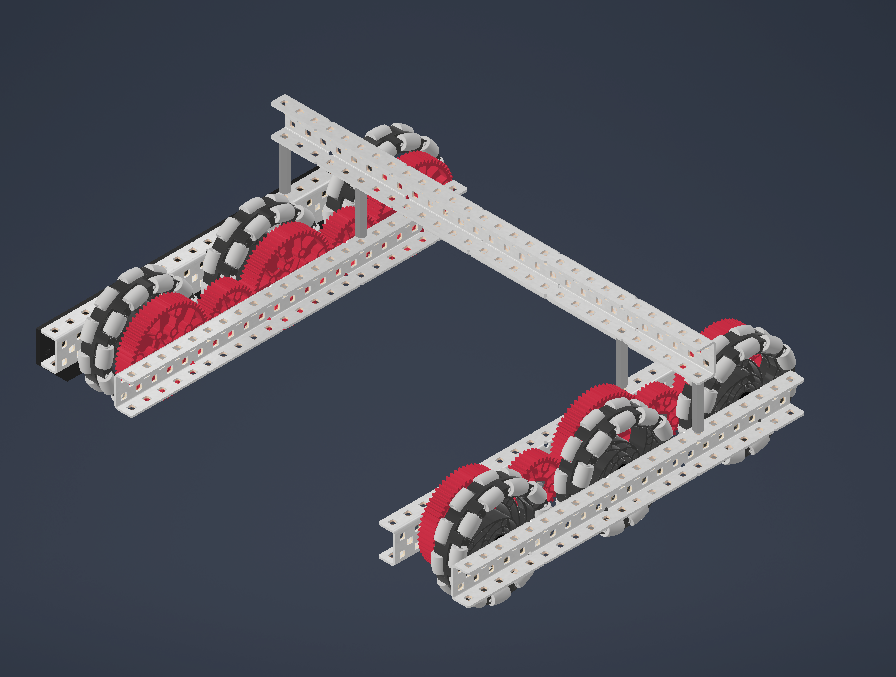
\includegraphics[width=0.45\linewidth]{images/15 cad/tank_ex.PNG} \hfill  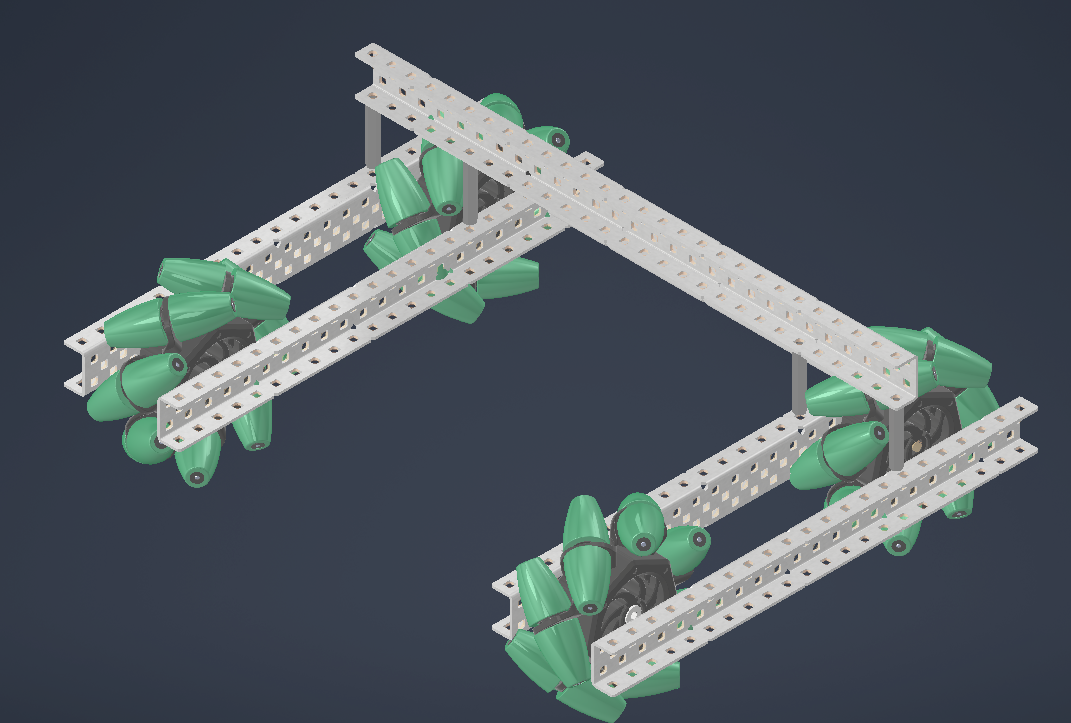
\includegraphics[width=0.5\linewidth]{images/15 cad/mechanum_ex.PNG} 
\end{figure}
\begin{figure}
  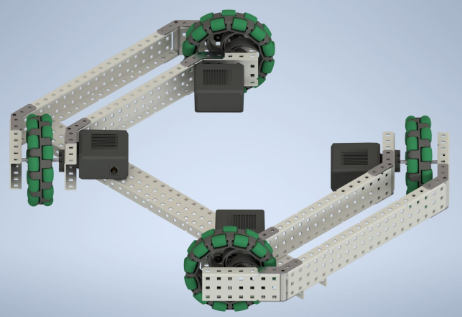
\includegraphics[width=0.45\linewidth]{images/15 cad/X-drive.png} \hfill  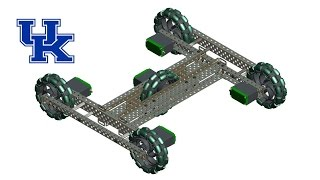
\includegraphics[width=0.5\linewidth]{images/15 cad/H Drive.jpg} 
\end{figure}
\begin{figure}
    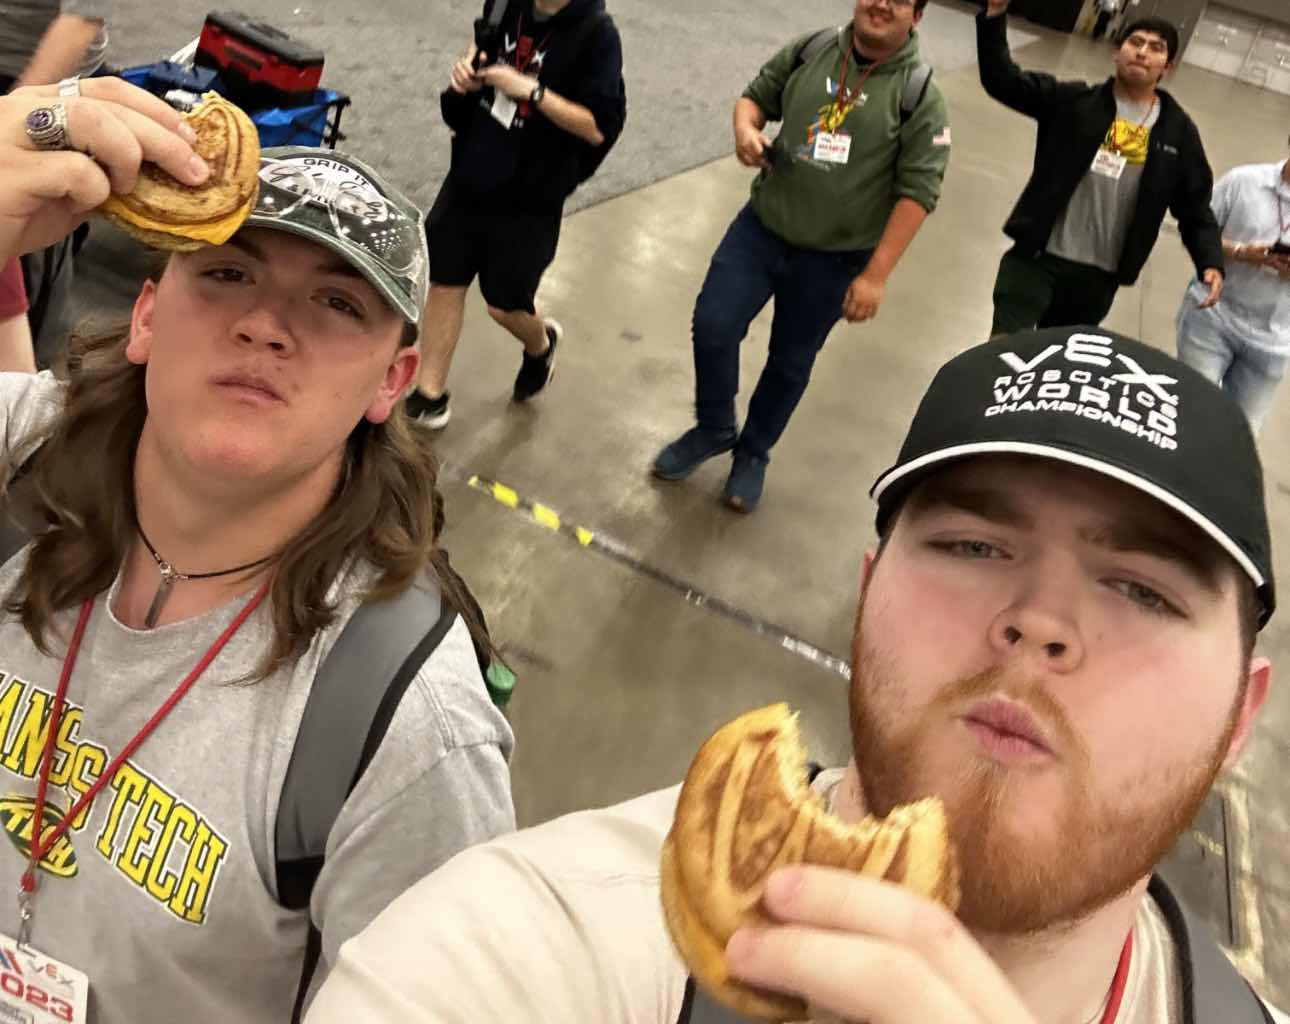
\includegraphics[width=0.5\linewidth]{images/july/mcgriddles.jpg} \hfill
    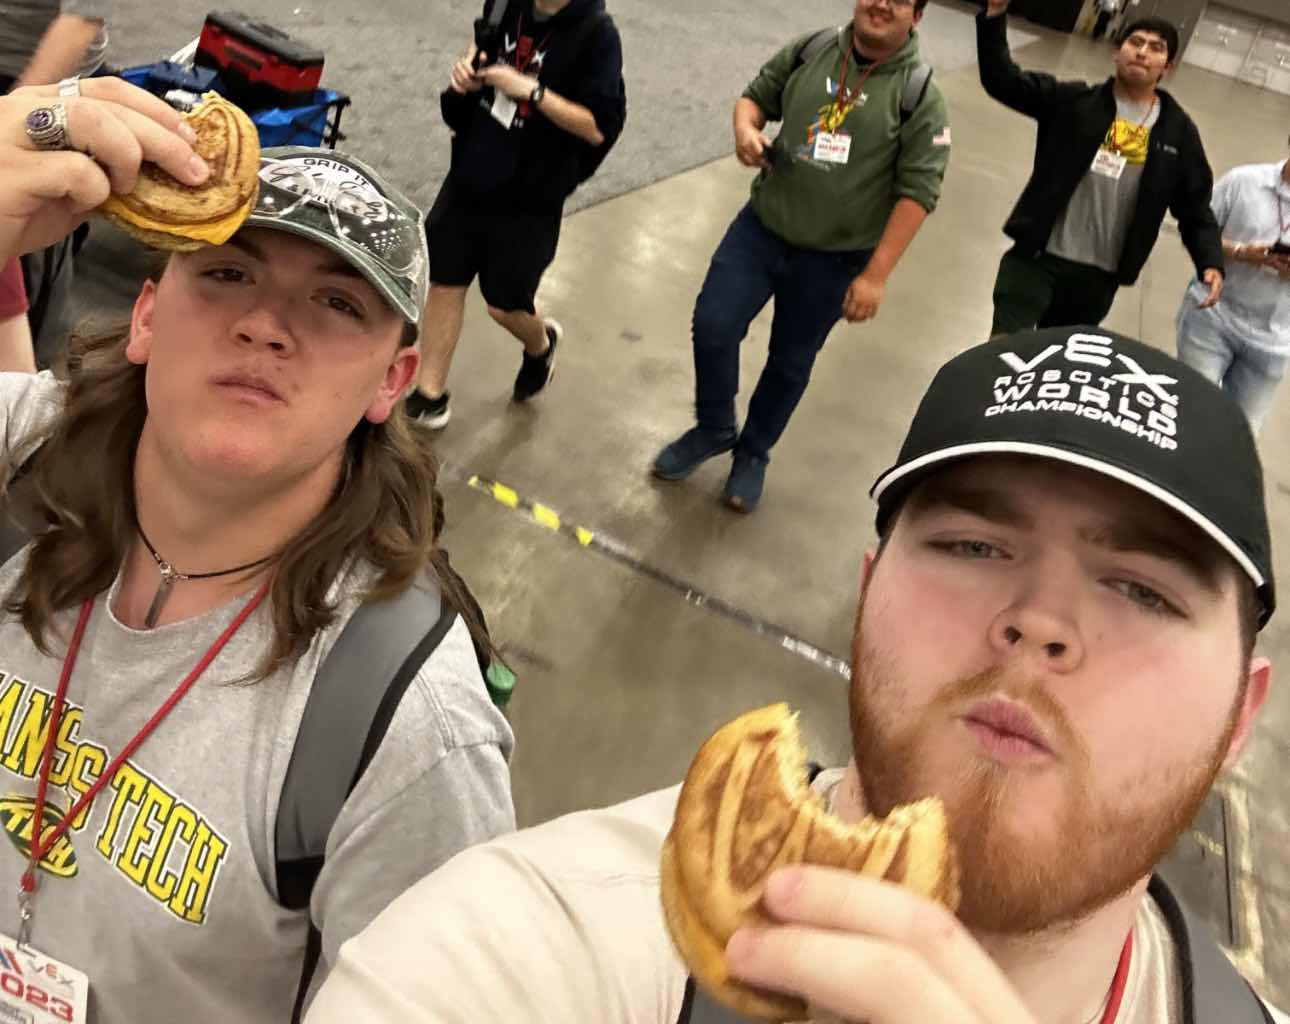
\includegraphics[width=0.5\linewidth]{images/july/mcgriddles.jpg}
\end{figure}

\begin{figure}
    \centering
    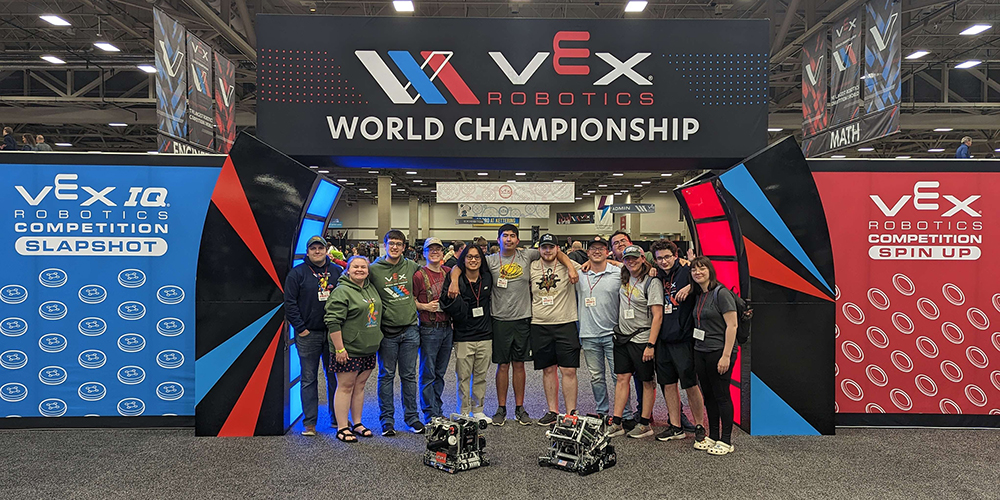
\includegraphics[width=0.5\linewidth]{images/july/2023worldchampionship.jpg}
    \caption{Absolute legends...}
    \label{fig:champs}
\end{figure}
\subsection{Triball Manipulation Brainstorming}
As obviously seen in \ref{fig:champs} ATUM's Family is pretty much going to win worlds and it is just a matter of when we get our trophy. 
\par Another major subsystem involves triball manipulation. Specifically, the kind
of triball manipulation that allows balls to be transferred from one match load zone on 
one side of the field to the other side of the field. This kind of manipulation in the past
has been done utilizing a launch system that launches a game element in the air to avoid
interference from opposing alliance bots on the ground. Though a subsystem can be developed to hold
triballs in the robot and have the robot drive to the other side of the field to score,
this would not be the premier choice for a high-scoring skills score. As such, we will 
discuss designs that can quickly move many triballs from one side of the field to the other.
Below is a design matrix ranking them: 
\insertmatrix{design-matrices/triball-manipulator-iteration-1.tex}{First iteration triball design matrix.}
\par The values for speed (and all categories) are rankings. Flywheel is
fastest, as it can allow continual launching. Catapult and sling rely on a
similar mechanism (tension) and are considered equal in this category. In last
is a claw which would require driving to move the triballs. \par The smallest
design would be a sling, because of its linear movement. Followed by a catapult,
since it moves in an arc. The flywheel design is next which, while it rotates
in-place, would involve the use of large wheels. The largest would be the claw
as it would near certainly involve a deployment mechanism. \par Accessibility
refers to how open the design is to maintenance. All of these designs require at
least occasional servicing (the flywheel may need new motors; catapult, sling,
and claw may need more bands), so this is worthy of consideration. Catapult
comes first in this regard, since the gearing can easily be placed toward the
outside of the robot; plus the fact it can be manipulated to get a better angle.
Flywheel and sling are next as they both lack inherently-inaccessible features.
The claw, comes last, again due to the cumbersome deployment system that would
be a necessity for such a design. \par For simplicity, catapult and sling are
tied for best since they rely on very similar mechanisms (tension) and since
Chris and Collin especially have experience with catapults. Next is the
flywheel, since there could potentially be more moving parts and the design
could involve tuning gearing, velocity control, and compression for consistency.
In last, again, is a claw since it would near-certainly involve a deployment
mechanism.
\pagebreak
\begin{figure}
  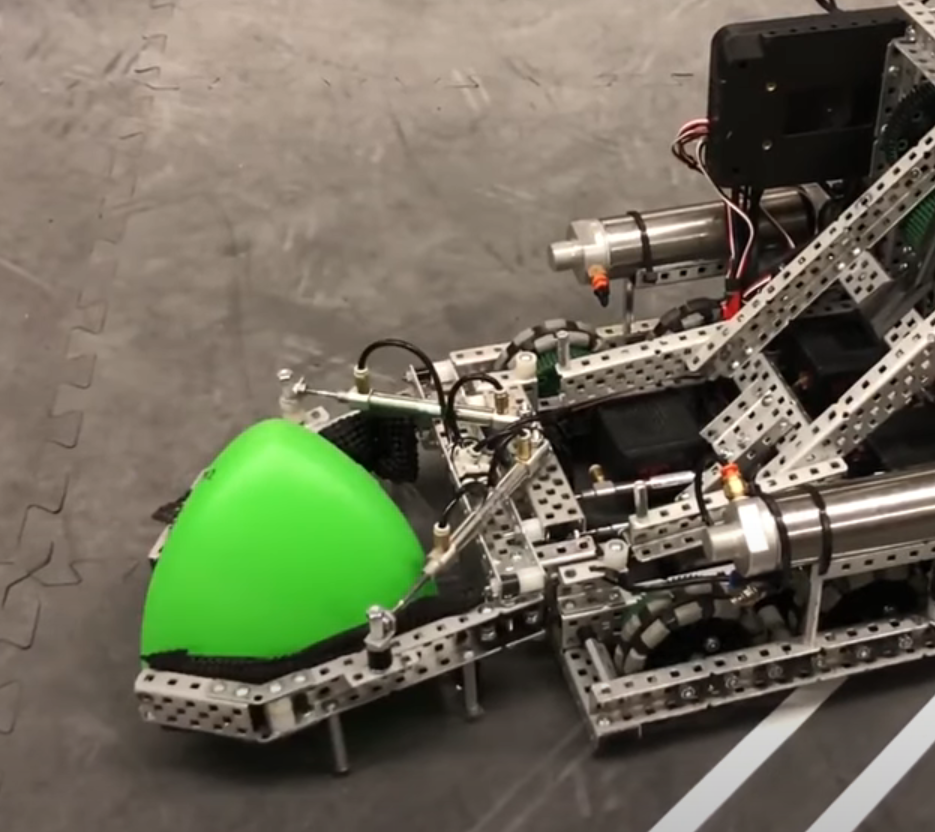
\includegraphics[width=0.4\linewidth]{images/15 cad/claw.PNG} \hfill  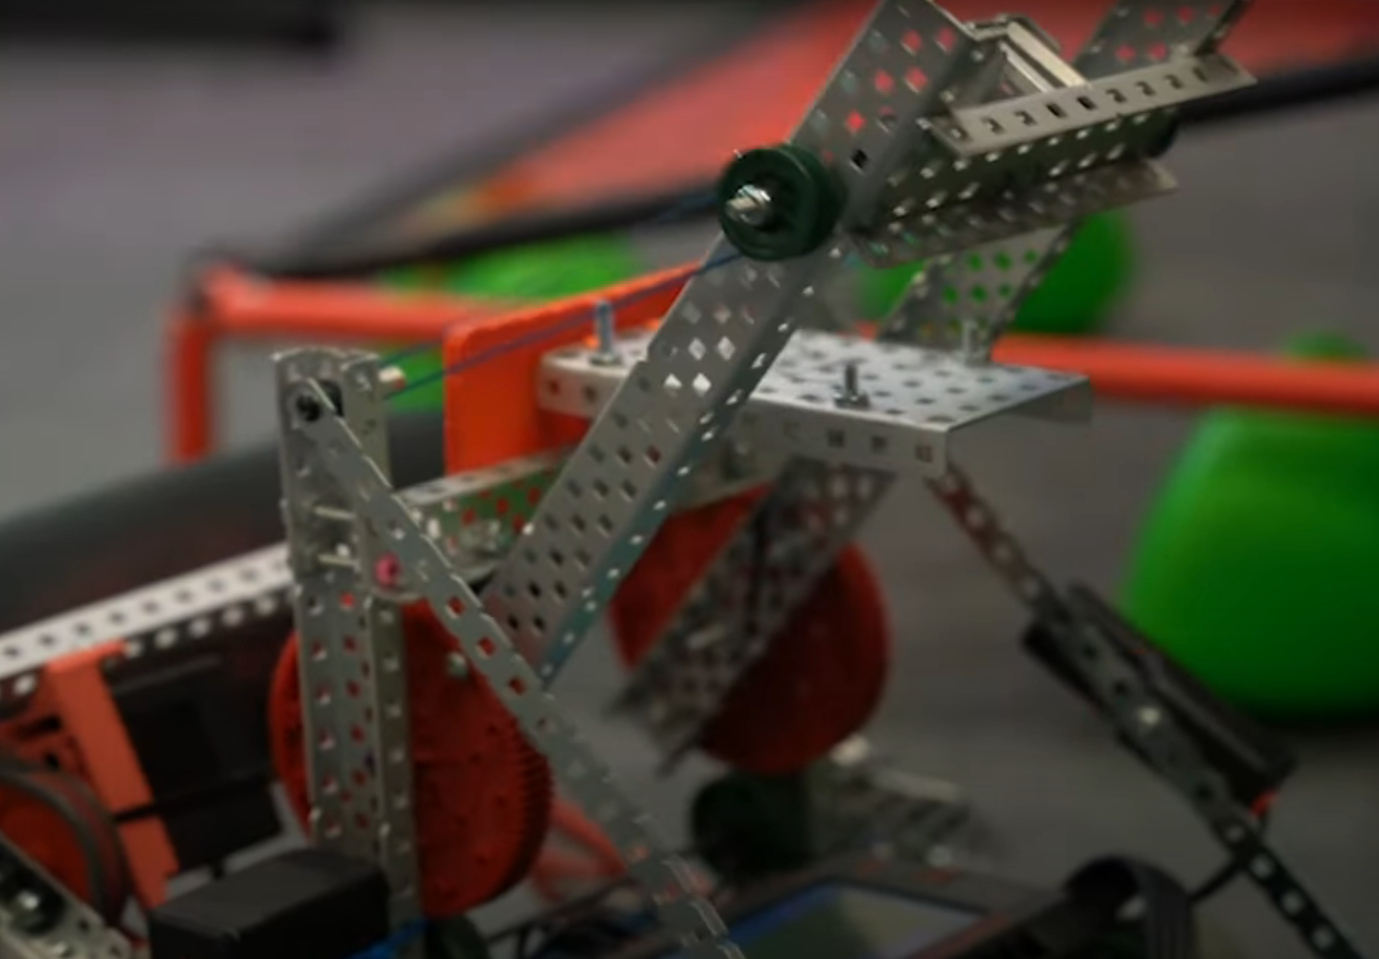
\includegraphics[width=0.5\linewidth]{images/15 cad/cataOwl.PNG} 
\end{figure}
\subsubsection{Examples of Triball Manipulation}
\begin{itemize}
  \item Left: Claw Mechanism \cite{bib:ClawPurdue}
  \item Right: Catapult Mechanism \cite{bib:Owl}
\end{itemize}

\pagebreak
\subsection{Intake Mechanism Brainstorming}
\par Though we have been ranking many major subsystems with a design matrix, we do
not know what intake mechanism will be the 'best' for triball intaking simply because
of the unique shape of a triball. Additionally, the design team and builders have no
prior experience with any form of triball-shaped game elements. However, we can still
present possible intake mechanisms to solve the challenge of intaking the Reuleaux-shaped
game element. We thought of 4 possible intake solutions:
\begin{enumerate}
  \item A series of compliant wheels mounted horizontally to intake a triball only from the top
  \begin{itemize}
    \item Pros
    \subitem -Easier to reach over match load zone
    \subitem -Wheels will last much longer than rubber bands
    \item Cons
    \subitem -Intake could get caught on the net since mounted above triball
    \subitem -Less compliance from wheels than stretchy rubber bands
  \end{itemize}
  \item A series of compliant wheels mounted vertically to intake a triball from both sides (think of car wash rollers)
  \begin{itemize}
    \item Pros
    \subitem -Two separate rollers working in tandem
    \subitem -Wheels will last longer than rubber bands
    \item Cons
    \subitem -Harder to reach into match load zone
    \subitem -Less compliance from wheel than stretchy rubber bands
    \subitem -Harder to power with only one motor
  \end{itemize}
  \item A series of banded sprockets mounted horizontally to intake a triball only from the top
  \begin{itemize}
    \item Pros
    \subitem -Easier to reach over match load zone
    \subitem -More compliance from rubber bands
    \item Cons
    \subitem -Rubber bands are less durable than wheels
    \subitem -Easier to get tangled on net or other robots
  \end{itemize}
  \item A series of banded sprockets mounted vertically to intake a triball from both sides (think of car wash rollers)
  \begin{itemize}
    \item Pros
    \subitem -Two separate rollers working in tandem
    \subitem -More compliance from rubber bands
    \item Cons
    \subitem -Rubber are less durable than wheels
    \subitem -Easier to get tangled on net or other robots
    \subitem -Harder to reach into match load zone
    \subitem -Harder to power with only one motor
  \end{itemize}
\end{enumerate}
While we could have put together a design matrix for possible intake choices, we thought it
was best to list out the positives and negatives and simply implement the best idea and compare them experimentally.

\subsection{Intake Arm Brainstorming Solutions}
Because of the rules involving match loading, we will require the use of an arm
to move the intake. There are two similar approaches and a unique approach that we consider:
\begin{enumerate}
  \item Four bar that has an intake mechanism mounted on top
\begin{itemize}
  \item Pros
  \subitem -intake stroke is highly adjustable
  \subitem -intake geometry is highly adjustable
  \item Cons
  \subitem -may be difficult to extend and retract the intake in a compact manner
\end{itemize}
  \item Chain bar with an intake mechanism mounted at the end
\begin{itemize}
  \item Pros
  \subitem -more control over the intake arm
  \item Cons
  \subitem -more points of failure with chain
  \subitem -harder to mount an intake mechanism at the end
  \subitem -match play may be compromised
\end{itemize}
  \item Hook mechanism that reaches over and pulls triballs into the robot
\begin{itemize}
  \item Pros
  \subitem -allows for a static intake
  \subitem -possibly pneumatic powered (reduces number of motors used)
  \subitem -lighter alternative
  \item Cons
  \subitem -less intake control when not match loading
  \subitem -hook mechanism will be useless outside of match loading
\end{itemize}
\end{enumerate}
Again, we decided against a decision matrix for this element of the design;
opting to instead to experiment to see the superior option.
\subsection{Plowing Mechanism Brainstorming Solutions}
\par Assuming that we can introduce all 44 match loads during the skills challenge,
we are left with the task of pushing dozens of triballs into our goal. The robots 
alone will not measure more than 15 inches and 24 inches respectively. The width of the
goal far exceeds 15 inches and exceeds 24 inches. Put simply, under the assumption
that both bots need to move a large amount of triballs into the goal, they will not be able to exceed the width 
of their drivetrains. The challenge at hand is to develop a way to temporarily 
extend the wingspan of the robots at a moments' notice to push more triballs around the field or into a goal.
This mechanism must be retractable, otherwise we would sacrifice maneuverability around the field; especially
around the low hang barrier. This concept of 'wings' was introduced by ACE 229V in late July \cite{bib:ACE} 
and our team believes that such a mechanism is required to score effectively. These are the possible
designs that should be considered:
\begin{enumerate}
  \item pneumatic actuating wings that are mounted in the front of the robot
\begin{itemize}
  \item Pros
  \subitem -more intuitive to use
  \item Cons
  \subitem -wings may fold in under pressure
  \subitem -wings have limited uses per match due to air pressure
\end{itemize}
  \item locking wings that get deployed from the top
  \begin{itemize}
  \item Pros
  \subitem -wings remain rigid under lots of force
  \item Cons
  \subitem -wingspan may be limited if the robot needs to go under the 12" hang barrier
  \subitem -wings have limited uses per match due to air pressure
  \end{itemize}
  \item motorized wings
  \begin{itemize}
    \item Pros
    \subitem -wings can deploy to a certain angle
    \subitem -wings can deploy indefinitely
    \item Cons
    \subitem -too bulky due to motors
    \subitem -costs too many motors for what they are used for
  \end{itemize}
\end{enumerate}

\subsection*{Endgame Brainstorming}
Once the last thirty-seconds of the match hits, teams are allowed to begin hanging from the elevation bars.
Since this is a good way to increase our score and winning chances, we were presented with the challenge of developing 
a way to get an efficient and high tier hang. Seeing that the elevation barriers only have 11.63" of clearance we needed
to come up with a mechanism that would still allow us to go underneath the barrier. Since we could design and build various ways of hanging,
we decided to brainstorm what would be the most feasible way to hang. As a team we came up with three different ways that we could potentially
elevate our robots at the end of the game: a tall pole hang, a short barrier hang, and the "buddy system." The first two options are the 
more standard approaches to achieving a hang that many teams will be doing. However, we want to do something that would not only stand out
but also allow both robots to reach as high as possible. We call this the "buddy system," which is where one robot drives onto and attaches
to the other and both hang from one contacting point of the pole. We once again opted out of creating a design matrix for this element of the 
design and took to looking at what option would seem to be the most reasonable.

\begin{enumerate}
  \item tall pole hang
\begin{itemize}
  \item Pros
  \subitem - maximizes elevation points
  \item Cons
  \subitem - requires a high torque mechanism 
  \subitem - can be hard to fit within size constraints of the short-barrier
\end{itemize}
  \item short barrier hang
  \begin{itemize}
  \item Pros
  \subitem - the fastest way to achieve a solid low level hang
  \subitem - easier to keep the robot within the clearance of the short-barrier
  \item Cons
  \subitem - can be outdone by other teams
  \end{itemize}
  \item the "buddy system"
  \begin{itemize}
    \item Pros
    \subitem - increases our chances of receiving the 1st and 2nd tier hang points
    \item Cons
    \subitem - reduces the amount of space we have on the 24" to mount other subsystems
    \subitem - decreases the amount of time left to score triballs
    \subitem - harder to maintain consistency
  \end{itemize}
\end{enumerate}

\section{15 Inch Design Selection}
This section will overview the design process of the first iteration of 15-inch
robot and will discuss all the subsystems contained within. Though processes, design
choices, building, and testing will be discussed.
\subsection{Vision}
\par The challenge with building a 15-inch robot is to do with its compact nature. We
must fit within a 15" x 15" cube in order for the robot to compete in any capacity.
However, once a match starts, the robot is able to expand past the 15" x 15" size
constraint. Upon starting the match, the robot can increase up to 36" horizontally
and can extend indefinitely vertically. This constraint is one that must always be
considered when designing any component of the robot. For this competition, these
are the features the team wants in the robot:
\begin{itemize}
  \item Triball pushing
  \item Match loading ability
  \item Elevation capability
  \item Clearing the elevation bar
  \item Ability to traverse middle barrier
  \item Triball holding
  \item Speed and torque
\end{itemize}
With these challenges laid out, we can design a robot with these constraints. Listing
these goals above, we can start assigning subsystems to them:
\begin{center}
  \begin{tabular}{| c | c |}
    \hline
    \bf{Subsystem}      & \bf{Goal}                         \\
    \hline
    Drivetrain          & Speed and Torque                  \\
    \hline
    Chassis             & Contain Subsystems                \\
    \hline
    Intake              & Manipulate Triballs               \\
    \hline
    Intake Arm          & Match Loading                     \\
    \hline
    Triball Manipulator & Moving Triballs to Offensive Zone \\
    \hline
    Endgame             & Elevation                         \\
    \hline
  \end{tabular}
\end{center}
\subsection{Drivetrain}
\subsubsection{Problem Statement:}
\par The team needs to design a mechanism capable of effectively maneuvering around the
field so that the robot can interact with game elements
\subsubsection{Solution Requirements:}
\begin{itemize}
  \item Must fit within 15" x 15" x 15" cube at the start of the match
  \item Needs at least 6 motors
  \item Must comply with $<$VUR4$>$ for any fabricated parts
\end{itemize}
\pagebreak
\subsubsection{Drive type:}
\par This year, our goal is to create a drive that can quickly move around the field whilst
still having the torque necessary to play defensive. Considering the many drives listed
in the initial design matrix, (Table 1.3), the most simple of the drives was the tank drive, scoring
a 5/5 for simplicity and was among the highest in climbing ability.
\insertmatrix{design-matrices/drive-iteration-1.tex}{First iteration drive train design matrix.}
\par  Last season, the team ran a mechanum drive on both the 15" and 18" robots for the first iteration. However, on the
15", the mechanums are simply too large and will prove time-consuming for an initial build. With
the tank being the most popular drive type and the most familiar drive type to the team, we
believe that a tank drive offers the most simple yet effective solution for the 15". This 
is due to the mechanum drivetrain being unable to have 6 wheels, which we believe is important
for traversing over the middle bar. The X and he H drive are simply too bulky for the 15".
Due to the comfort and familiarity with the tank drive, the 15" design will be a tank drive.
\subsection*{Speed and Torque:}
\subsubsection{Problem Statement:}
\par Identify a desirable wheel size and gear ratio for the robot
\subsubsection{Solution Requirements:}
\begin{itemize}
  \item Must have 6 wheels
  \item Must be faster than a direct-drive 200RPM green cartridge
  \item Must be powered by a 600RPM cartidge
\end{itemize}
\pagebreak
\subsubsection{200RPM vs 600RPM:}
\par There are many combinations of wheel sizes and gear ratios. However, with the 15" robot,
we want a drive that will be compact and balanced. Utilizing a 200RPM green cartridge, we 
would need to have a speed ratio on the gear train. This is not ideal for a 6-motor drive.
Additionally, green cartridges have more gear reduction internally, thus they have more
friction. Blue cartridges have less of a gear reduction thus have less friction from there
being less moving parts. Moreover, we will be able to gear the drive for torque, resulting
in more compact gearing. This is ideal for a compact drive base.
\subsubsection{Wheel Size:}
\par For the foreseeable future, the team only has access to 4" omnidirectional wheels and
3.25" omnidirectional wheels. Though 4" omnidirectional wheels are more ideal for climbing the 
barrier, 3.25" offers a more compact form factor for the 15" constraint. Our driver
last year was very comfortable with 333RPM at 3.25". 3.25" seems only rational for the 1st
iteration
\subsubsection{The Design:}
After many hours of cadding, the following was concluded:
\begin{itemize}
  \item The drive will be 360RPM powered by a 36T gear driving a 60T gear for torque
  \item It will have 6-omnidirectional wheels
  \item the length of the entire drive will be 13.5" to give headroom for any mechanisms
\end{itemize}
\par Below is the basic ratio of the drivetrain and the beginning of the chassis CAD:
\insertimage{images/15 cad/15driveratio.PNG}{0.5}
\pagebreak
\par The CAD file just shown will have the 36T powering the 60T gears for a torque ratio.
With 600RPM motors, it will result in a 360RPM ratio at 3.25"
\subsection{Chassis:}
\subsubsection{Problem Statement:}
\par Design a chassis robust enough to withstand the shock of constantly climbing over the
barrier and easy enough to build on
\subsubsection{Solution Requirements:}
\begin{itemize}
  \item must be no longer than 13.5"
  \item does not have open ends
  \item does not twist
  \item has space for subsystems and sensors
\end{itemize}
\par With the ratio already discovered, we simply need to create a strong base
around the wheels. Last year, our 18" robot suffered from not having a support that ran
across from end to end. We only had one c-channel that ran across from outer chassis to outer chassis, and it did not work as desired. Coming up with a design for the 15", this design was created:
\insertimage{images/15 cad/Chassis_Basic.pdf}{0.2}
\pagebreak
\par Note that there are two c-channels that run from outer-end to outer-end. One is
in the rear of the robot, and the other is near the front above one of the 36t gears. This greatly
improves the rigidity of the chassis. The front and back of the chassis will eventually have
reinforcements, but the chassis should now be ready to be tested.
\subsubsection{Testing:}
\subsubsection*{Problem}
This basic design was built with only 4 motors and some interesting observations were noted:
\begin{itemize}
  \item The chassis is susceptible to skewing(the entire chassis can potentially be pointing slightly left or right)
  \item when skewed, it may induce friction
  \item one side of the drivetrain was noticeably stiffer to move than the other
\end{itemize}
\subsubsection{Solutions:}
After constructing the drivetrain, we tested the wattage that was being pulled from both the left and right
side of the drive. Seeing that the chassis and its components are one of the must fundamental elements of the 
design, we wanted to obtain the lowest amount of friction possible. We ran a wattage test on the left side of 
the drive by running the motor at max speed. We found that the left side was pulling about 0.78 Watts. Then we
tested the right side of the drive and found that it was pulling around 1.5 Watts. Seeing that the left side was 
pulling a decent wattage, we tested the right side of the drive by swapping over the motors from
the left side, reducing teflon spacing, and creating 3d printed chassis support blocks. Below is a table that shows these test.  
\insertimage{images/15 tables/drivetrain test.PNG}{1}
After running this test, we were able to deduce that when reducing the spacing on the right side of the drive 
it began to pull a wattage closer to the left. We realized that the motors were performing properly and were not the issue.
We then reduced the teflon spacing and found that it began to pull less watts. Since we were still not happy with the results,
we decided to square the chassis off with 3d printed support blocks. After doing so, both the left and right
side began to pull the same wattage. The 3-D printed block is shared among both the 24" and
the 15" and this is how it interacts with the chassis:
\insertimage{images/24cad/24_notebook_1.pdf}{0.2}
\par Much like some vex sensors, the rounded square pieces snap inside the c-channel holes and essentially
make the c-channels move all as one. With four of these on the chassis, the chassis no longer suffered from 
skewing like before.
\pagebreak
\subsubsection{Competition Chassis}
\par Following the development and installation of all other subsystems, the chassis of the robot is displayed below:
\insertimage{images/15 cad/Chassis_Complex.pdf}{0.21}
The follwing items are installed:
\begin{itemize}
  \item Sleds
  \item Skirts
  \item Motor Stack Chassis Support
  \item Brain
  \item Battery
\end{itemize}
\subsection{Wings}
\subsubsection{Problem Statement:}
\par Develop a mechanism for pushing triballs that resembles 'wings'
\subsubsection{Solution Requirements:}
\begin{itemize}
  \item Fit within the chassis c-channel
  \item Does not allow backtracking
  \item Powered by a double acting piston and not a motor
\end{itemize}
\subsubsection{Compact Front Wing Prototype (Iteration 1)}
\par As discussed in our vision of the 15" robot, we want to be able to have front-mounted
wings on the robot so we can push triballs. Before designing the intake, we believed it would
be best to come up with a wing mechanism that can sit parallel to the outer-chassis
when not in use. Taking inspiration from Robokauz Robotics 21417A \cite{bib:Robokauz} we liked their idea of a 
wing that is locking, thus we prototyped a design:
\begin{figure}
  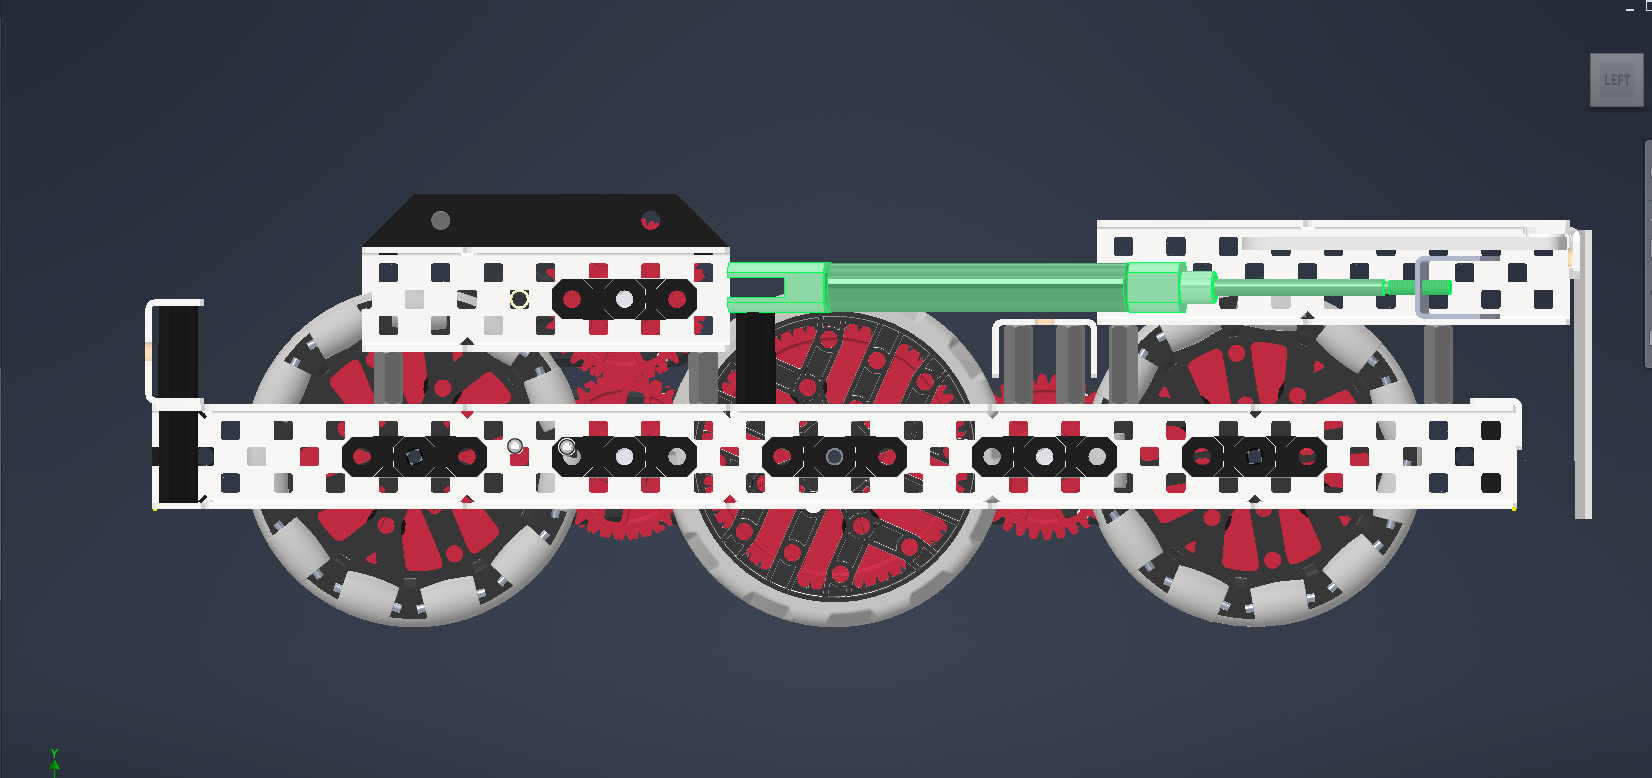
\includegraphics[width=0.5\linewidth]{images/15 cad/15newsider.PNG} \hfill  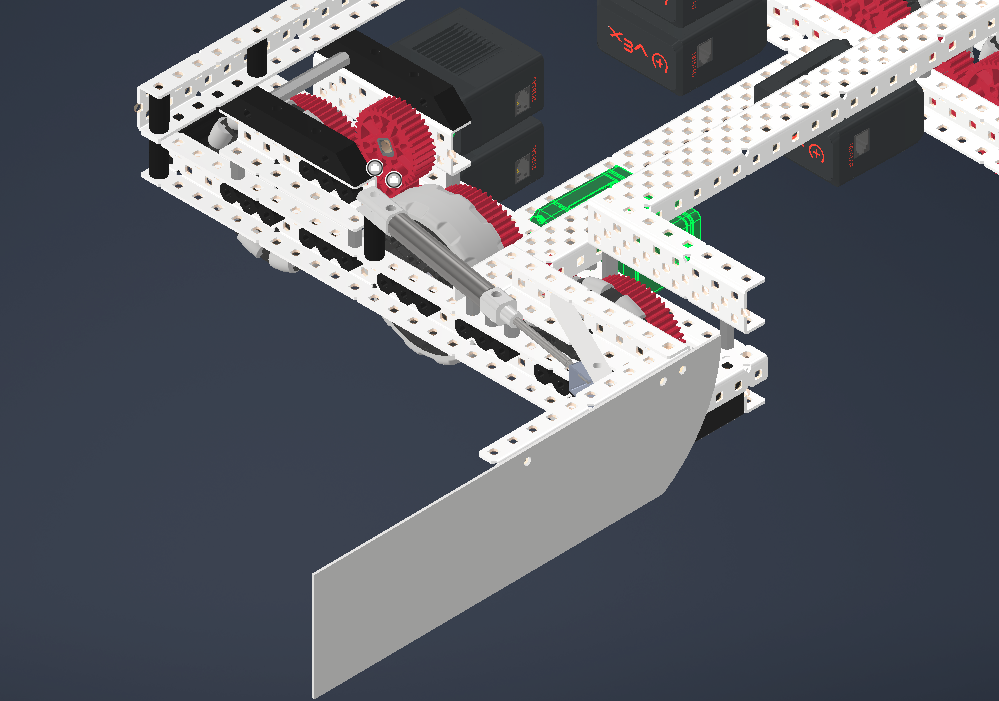
\includegraphics[width=0.5\linewidth]{images/15 cad/15newside.PNG} 
\end{figure}
\par The large flat piece attached to the angle piece that slides out is a prototype for a 
piece that will allow the robot to lift when driving towards the middle barrier. Planned to 
be cut out of a piece of polycarbonate, it will open with the wing assembly.
\subsubsection{Testing: Iteration 1}
\subsubsection{Problem:(Iteration 1)}
\par This design was built and tested without the polycarbonate piece in the CAD rendition. 
The following observations were noted:
\begin{itemize}
  \item Though the CAD allows the wing to theoretically deploy, the force required was underestimated
  \item The 2-wide c-channel needed to be expanded to a 3x c-channel
\end{itemize}
The following tests scenarios were tested and listed in the table below:
\insertimage{images/15 tables/front wings test.PNG}{0.8}
In this table, we tested to see how many (out of five actuations) times that the wings would deploy.
We tested the wings without any aid and noted that they were not able to deploy at all. We then
tested with rubber bands, springs, and a combination of both. While the number of deployments slightly 
improved, it began to make the design too bulky and did not seem practical to try and make this design work.
\subsubsection{Rear Wing Prototype (Iteration 2)}
\subsubsection{Problem Statement:}
\par Design a new wing mechanism that is mounted in the rear of the robot
\subsubsection{Solution Requirements:}
\begin{itemize}
  \item Wings must not require the removal of functional subsystems
  \item Wings must be rigid
  \item Wings must keep robot in size
\end{itemize}
\par With the majority of the bot built, making the wings work in the front was no longer
possible since there are major subsystems that can not relocated without an entire rebuild.
\par Though not what the team envisioned, drop-down wings seemed to be possible
if mounted in the rear of the robot. Mounting a c-channel on a hinge on the rear of the
robot, we began to experiment with placement of the pistons and discovered a possible mount:
\insertimage{images/15 cad/dropdownproto.jpg}{.08}
\par With the location discovered, the CAD was updated with the new mounting positions
considered. The following wing was designed:
\insertimage{images/15 cad/WIngDropDownFinal.PNG}{.4}
\subsubsection{Testing: Iteration 2}
\subsubsection{Problem:}
\par Upon building and testing the new wings, one many observations were made:
\begin{itemize}
  \item The SMC pistons were not strong enough for that mounting position, but they could deploy the wings
  \item Swapping pistons resulted in the wings no longer deploying
\end{itemize}
\par With slightly stronger double acting pistons installed, they did not actuate at the first try.
We thought it was too much friction in the hinge, but even with a rebuild, they did not improve.
We ran the following tests listed below:
\insertimage{images/15 tables/rear wing test.PNG}{0.8}
We tested the rear wings exactly how we tested the front wings. Just like the front wings, the rear wings
were unable to deploy without any aid. However, as we ran the test by adding springs, bands, and a combination
of both the results increased drastically. Since we are now working on the rear of the robot, we had quite
a bit more workroom. Therefore, we decided to keep this design and pair it with rubber bands and springs
to get a more consistent and faster wing deployment. 
\subsection{Intake}
\subsubsection{Problem Statement:}
\par Develop an intake solution that can retrieve match loads
\subsubsection{Solution Requirements:}
\begin{itemize}
  \item Intake must be able to reach over match load barrier
  \item Intake must start within 15" x "15 x 15" area at the start of the match
\end{itemize}
\subsubsection{Intake Iteration 1:}
\par Due to the strange shape of a triball, we believe that a top-down rubber band and sprocket solution
is going to be a more viable option for the 15" simply due to the size constraints. The team believes
this based off of a basic implementation of a two-flex-wheel intake by Aubie 1 \cite{bib:Auburn}. This
is further reinforced by the excellent early-season implementation of a band-and-sprocket intake by
ACE 229V \cite{bib:ACE}. Moreover, a sprocket intake mounted on a four-bar mechanism would
allow our robot to retract the intake inside it. The initial design of the intake was created in CAD
using measurements of the match load barrier and triball height. The goal was to have the rubber bands
graze the tip of a triball to suck a triball into the robot.
\pagebreak
\par A very popular mechanism from the 2017-2018 Vex Robotics Competition was used for reaching
over a similar game element. A mobile goal mechanism from in the zone would keep a mobile
goal inside the robot as seen in a demonstration from 20785B \cite{bib:Mobilegoal}. Though not exactly
applicable to this year's challenge, the idea of a motorized intake retraction system would
seem ideal for match loading. 
\begin{figure}
  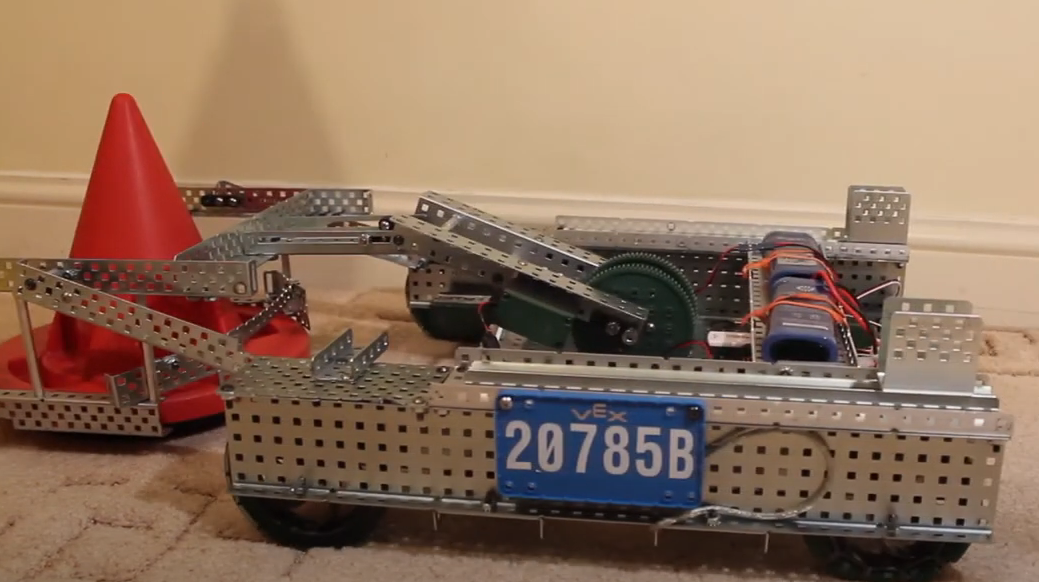
\includegraphics[width=0.5\linewidth]{images/15 cad/IntakeEx.PNG} \hfill  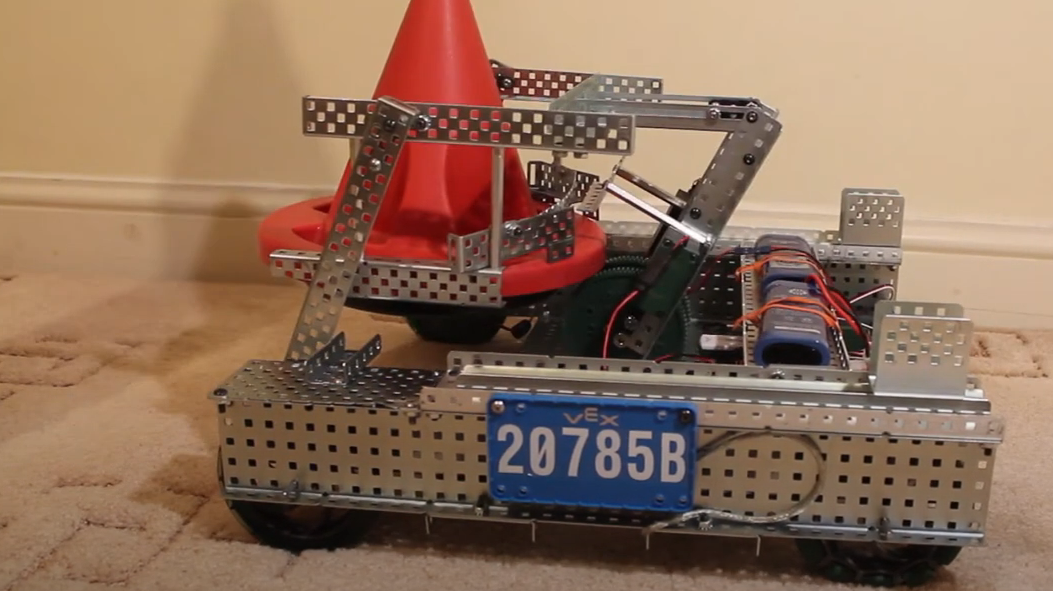
\includegraphics[width=0.5\linewidth]{images/15 cad/IntakeEx2.PNG}
\end{figure}
\pagebreak
\par With these design considerations in mind, iteration 1 of the intake was designed and built
with a 200RPM intake speed:
\begin{figure}
  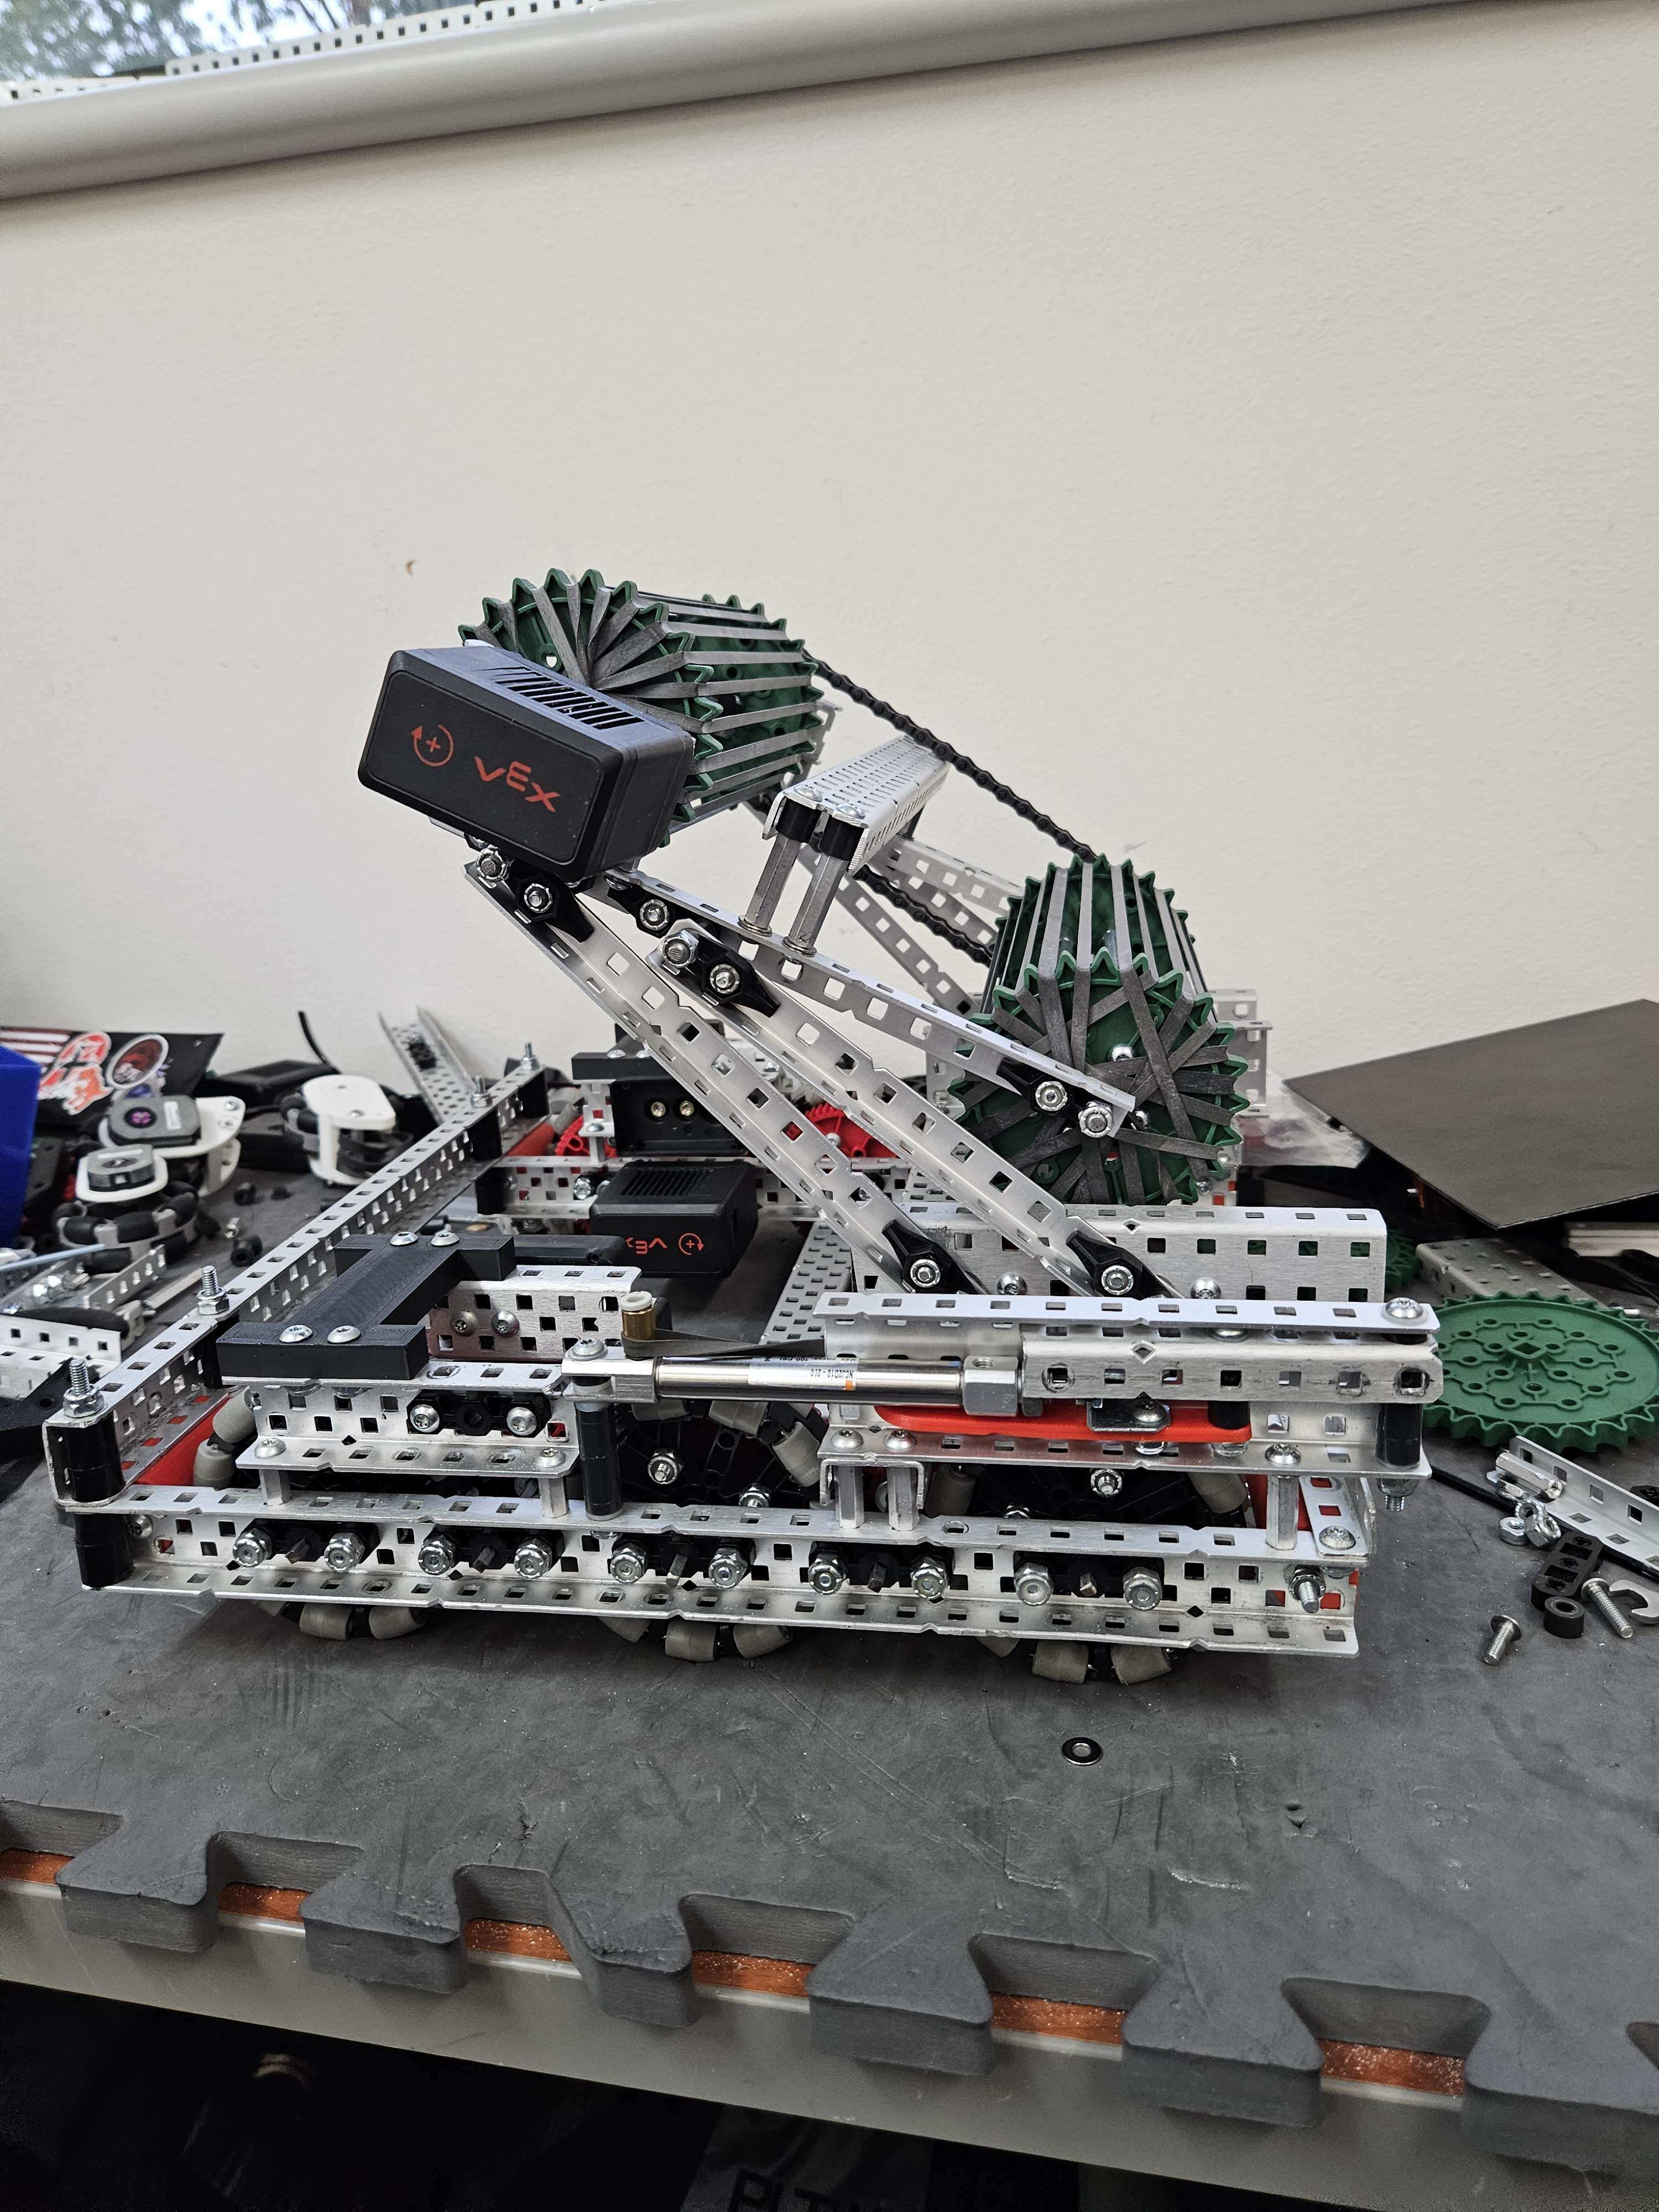
\includegraphics[width=0.4\linewidth]{images/15 cad/intake original.jpg} \hfill  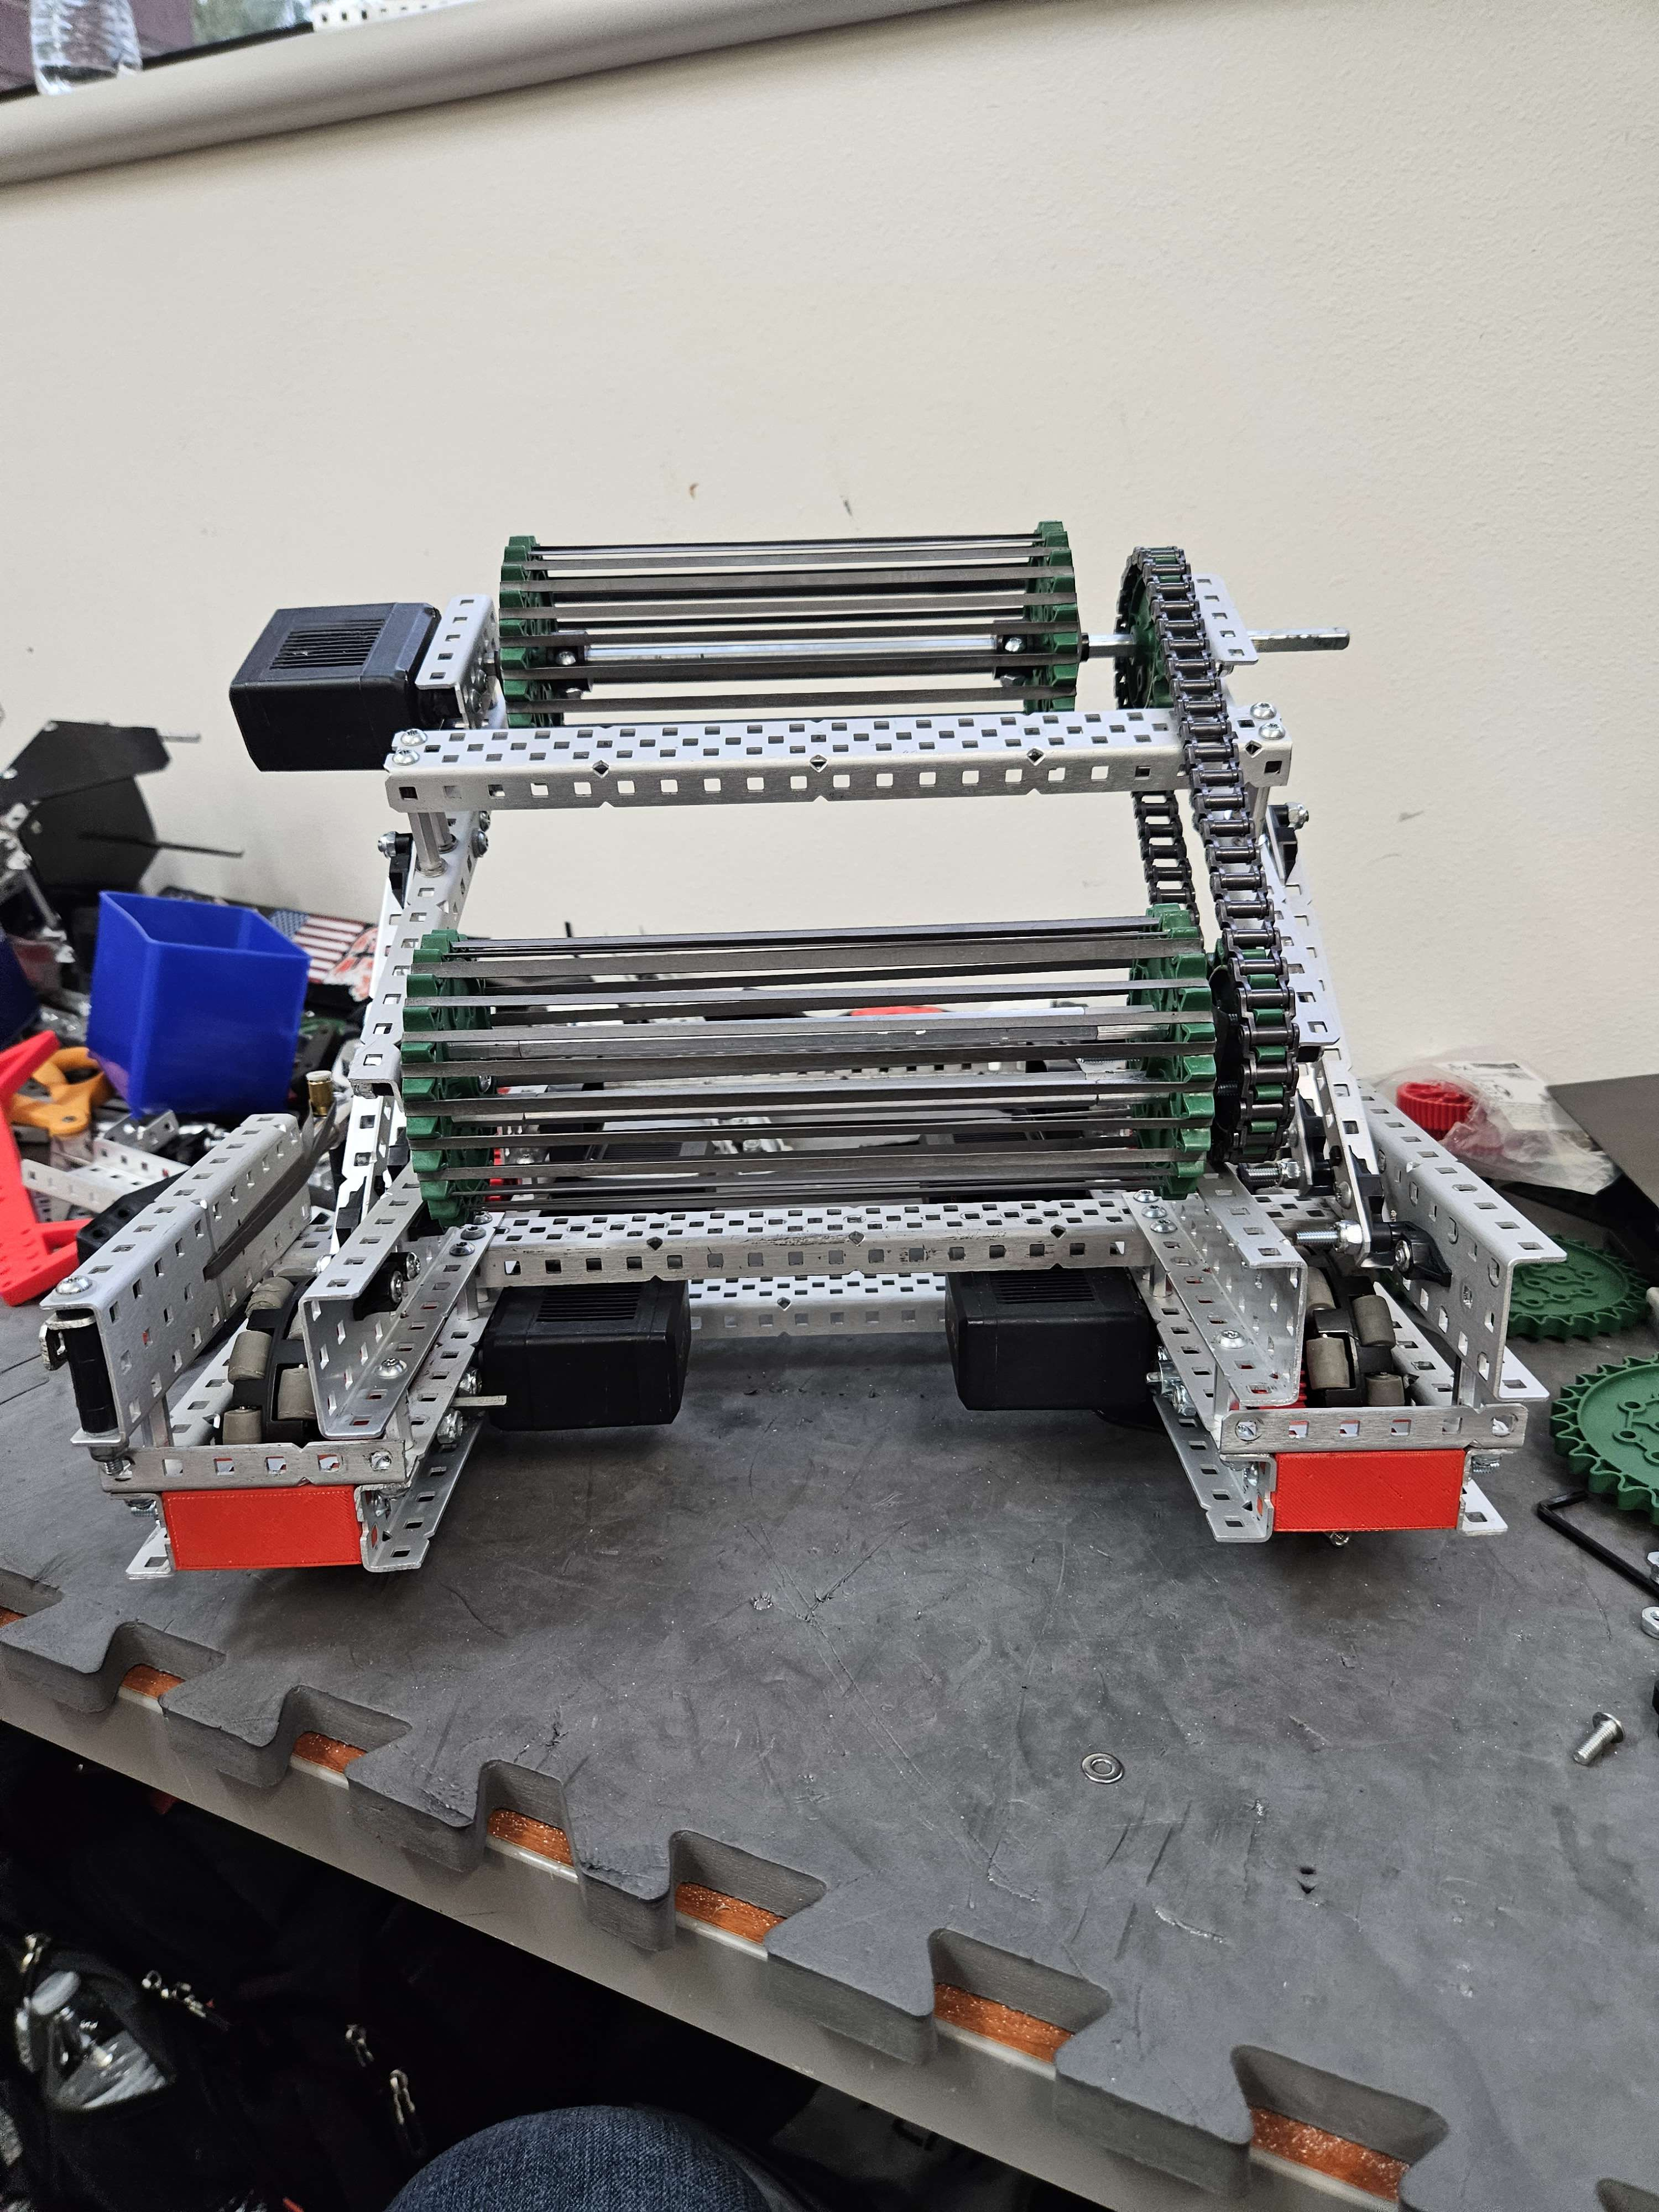
\includegraphics[width=0.4\linewidth]{images/15 cad/intake original front.jpg}
\end{figure}
\par This is the CAD of the intake built. To keep the intake as wide as possible and in size, note that the intake is
not centered with the chassis. Rather, the intake is shifted over to make sure that the robot
remains within the size limit. This intake was designed to allow many modifications to the angle and
length of the stroke when reaching out.
\subsubsection{Testing Iteration: Trial and Error}
\par An intake for this season will require lots of trials and tests to get it in a usable
state. Even with a CAD model of the field and match load zone, CAD can only go so far.
Thus, Iteration 1 was an immediate failure after multiple tests.
\subsubsection{Problem:}
\par Intake iteration 1 did not work at all to retrieve match loads. The following was observed:
\begin{itemize}
  \item Triballs simply spun on the match load barrier when intaked
  \item The triballs immediately hit on the front sprocket axle when intaking
  \item The intake had to be perfect positioned (needed a hard stop)
\end{itemize}
\pagebreak
\subsubsection{Solutions:}
\par These solutions were proposed
\begin{itemize}
  \item The intake needed a larger sprocket so that the triballs had more leeway when being intaked
  \item There was more room for error with more rubber band travel. 
  \item Look into moving the intake out
\end{itemize}
\par Given the observations, the following proposed solutions were tested and split into two cases:
\subsubsection{Case 1: 200RPM}
\subsubsection{Case 2: 600RPM}
\par The following tests were were conducted and listed in the tables below:
\insertimage{images/15 tables/iteration 1 200 speed intake.PNG}{0.8}
\insertimage{images/15 tables/iteration 1 600 speed intake.PNG}{0.8}
\par Some intresting observations were made with the tests
\begin{itemize}
  \item Triballs behave more like a ball at higher rolling speed
  \item Larger sprockets allows more room for error while intaking
  \item Larger sprockets allows for the triball to be intaked at awkward positions
\end{itemize}
\par The combination of both a larger sprocket and a faster intake speed yielded
by far the best results in each case. Overall, the 200RPM motor on the intake lacked the speed
required to intake triballs as effectively. Data from these tests gave us critical information.
At the point we are now, all we need is some sort of mechanism to quickly extend and retract the intake, so the robot can intake in succession.
\subsubsection{Intake Retraction and Extension: Iteration 2}
\subsubsection{Problem:}
\par Intake speed and material discovered, but we need to find a way to have it retract
completely inside the robot to start in size at the start of the match. This mechanism must also 
be able reach out over the barrier.
\subsubsection{Solution Requirements:}
\begin{itemize}
  \item Intake needs to be able to retract completely inside the bot
  \item Intake needs a hard stop to that the extension mechanism does not overextend
  \item robot needs to be able to keep a consistent extension/retraction after multiple uses
\end{itemize}
\par Immediately, we identified that we can power the intake retraction with either
pneumatics or motors. Both have their respective pros and cons:
\begin{enumerate}
  \item Pistons:
  \subitem -Limited use  (con)
  \subitem -Compact (pro)
  \item Motor:
  \subitem -Much more use and adjustability (pro)
  \subitem -Will be difficult to power with only one motor (con)
  \subitem -Not as compact (con) 
\end{enumerate}
\pagebreak
\par We found there to be more individual cons to motors than to pneumatics. However,
simply because there are more cons for motors does not rule them out as a design choice.
Motors, as big and bulky as they are for this specific application, offer one major upside: adjustability and repititon.
A piston-powered intake stroke is not ideal for our use case due to the limited amount of uses 
per match. Limited use is especially important for skills, where we believe it is critical
that we get all 22 match loads as fast as possible. Moreover, prototyping a motor-powered
arm will be much more simple than trying to tune intake stroke with only a 2-inch double-acting
piston. Additionally, we do not have many pistons to use as we are saving them for wing mechanisms.
So in the interest of time we will choose to experiment with a motor-actuated intake.
\subsubsection{Rotational to Linear Motion: Slider-Crank Mechanism}
\par There are many mechanisms that turn rotational motion to linear. Just recently, discussing
team 20785B's mobile goal design \cite{bib:Mobilegoal}, was an example of rotational motion to linear motion. Their 
mechanism follows the same principle as a rod-and-piston within an engine. It can be illustrated 
in this diagram below \cite{bib:RotarytoLinear}:
\insertimage{images/15 cad/SliderCrank.PNG}{0.75}
\pagebreak
\subsubsection{Rotational to Linear Motion: Linear Slide}
\par Another mechanism used for converting rotational motion to linear motion is
the linear slide mechanism. A linear slide involves a gear driving a linear slide that
has a rack gear attached to it. Below is an example of a slingshot mechanism powered
by a linear slide \cite{bib:Linear}:
\insertimage{images/15 cad/LinearSlide.png}{0.4}
\par This mechanism has not been too popular in the last few seasons because of the
 Vex hardware limitations. Though great for repetitive tasks, the Vex library of parts
 is rather lacking in geometry when it comes to the linear slide rail and mounting system.
 Additionally, all linear slide components that Vex makes are steel. With these considerations,
 we can create a design matrix for choosing the mechanism:
\insertimage{images/15 tables/intake retract matrix.PNG}{0.8}
\par Note that compatibility is constant, thus a lower total is better. We will move 
forward with prototyping a motor actuated intake retraction system.
\pagebreak
\subsubsection{Testing: Iteration 2}
\par No CAD assembly has been created for the intake retraction mechanism, but we were able
to prototype a possible mechanism:
\insertimage{images/15 cad/intakearmproto.jpg}{0.08}
\par Using a 60t gear as a universal crank-arm, we discovered that we could essentially
create a slider-crank mechanism out of a 60t gear, a screw joint, and have an aluminum angle
connect to one of the intake arms. Spinning the 60t gear, we get a complete intake/retraction
stroke by spinning the 60T gear a few degrees. The following prototype was built:
\insertimage{images/15 cad/intakearmproto2.jpg}{.08}
\pagebreak
\par With the 60t gear being powered by a single 200RPM motor, we discovered the following:
\subsubsection{Problem:}
\par The intake now has a hard stop and can extend and retract, but it is plagued by many
issues:
\begin{itemize}
  \item One single 200RPM motor does not have the torque to move the intake forward
  \item By moving the aluminum angle connection up, the desired intake extension is not as far as desired. more torque=less travel and less torque=more travel
  \item When the motor can move the intake, it is done too fast, making it unusable
\end{itemize}
\subsubsection{Solution Requirements}
\begin{itemize}
  \item Intake arm must retract and extend quickly, but must not be so fast that it is unusable
  \item Intake mechanism must have enough torque to reach desired intake extension/retraction
  \item Intake must retract nearly into the robot to remain in size at the start of the match
\end{itemize}
\subsubsection{Intake Geometry Solution}
\par While testing we discovered that our 4-bar intake linkage will extend much more if the aluminum angle
connected to one of the intake arms is connected closer to the axis of rotation. Think of a wrench for example.
If you want to break a bolt loose that is incredibly tight, you would use a breaker bar. However, once
broken loose, using a long bar to undo a bolt that is no longer tight would take an incredibly long time. Conversely,
if you have a really tight bolt, and you use a smaller wrench to break it loose, you do not have the 
torque required to break it loose. The rational thing would be to break a bolt loose with a breaker bar, then swap to 
your smaller wrench to unscrew the bolt much quicker than with the breaker bar. This concept also applies for
the intake. By measuring how far the intake needed to extend and recording the distance, we created
a CAD model of the robot in its current state and discovered by trial-and-error that the 4th hole
of the intake arm of the 4-bar linkage of our intake works the best with the displacement created by
spinning the 60t gear about 180 degrees.
\subsubsection{Torque Solution}
\par We noticed that the 200RPM motor not only spun too fast, but it had no torque at all. This does not 
surprise to us, as the motor powering the intake is directly driven. Going with the most basic approach, we opted to
change the motor to a 100RPM red cartridge One motor alone was still not enough, so we mirrored what we had and tested
the intake.
\par Testing with both motors was a success. The intake extension speed was fast, but still usable.
Retracted, the intake was now in size. Extended, the intake was now able to reach over the match load
barrier and intaking triballs in succession.
\pagebreak
\subsubsection{Moving the assembly to the rear}
\par As though we successfully prototyped a solution, we did the mounting solution at 
the time of prototyping was taking up valuable space in the center of the robot:
\insertimage{images/15 cad/intakePreMove.jpg}{.08}
\par Positioned directly above the center of the robot, it would be extremely difficult and time-consuming
to develop a shooting mechanism for the robot. Mounting the motors as far back as possible, we simply
extended the C-Channel to connect with the rear. This opened up lots of room in the middle of the chassis:
\insertimage{images/15 cad/intakePreMovevsOld.jpg}{.08}
\subsection{Flywheel}
\subsubsection{Problem Statement}
\par Design a mechanism capable of manipulating intaked triballs obtained from either the match load zones
or the field tiles to score
\subsubsection{Solution Requirements}
\begin{itemize}
  \item Mechanism must be able to traverse under hang barrier and start within 15" x 15" x 15" at the start of the match
  \item Mechanism must be able to quickly interact with intaked game elements
\end{itemize}
\par Coming from last season's game: Spin Up, our builders are incredibly familiar with flywheel and catapult
mechanisms. Having identified the strengths and weaknesses of many possible shooting mechanisms in the initial
design overview, we can reflect on the design matrix:
\insertmatrix{design-matrices/triball-manipulator-iteration-1.tex}{First iteration triball design matrix.}
\par A catapult and sling are the most compatible with a smaller robot. However, we deduced that the flywheel
was the flywheel was the fastest for individual game element firing in succession. This was due to the lack of tension.
Tension is a critical component in sling and catapult mechanisms. Thus, if we were to use a catapult, we would
need to shoot it and wait until it reset and repeat. Familiar with flywheels and catapults from the Spin Up season, we know that
a properly-built flywheel will always be faster at shooting single game elements in succession.
\par Where the catapult excels is in shooting multiple game elements at once. Such as in last years' game, where the
robot could possess up to three game elements at a time. This season differs greatly however, as the robot can only 
possess one game element at a time. This makes a flywheel much more favorable for VEX U, as our robot
needs to retrieve triballs placed in the match load zone. The robot must then reach out, intake the ball, then shoot it
out to its respective offensive zone to score. Introducing a catapult reload time into 22 match loaded triballs, and
we could lose potential seconds.
\par Building a catapult is something that the build team is familiar with. We know that a catapult is incredibly simple to
implement. Thus, we will decide to prototype a flywheel solution for our robot. Though it may prove troublesome, if 
implemented correctly, a flywheel could be one of the fastest match loading solutions for this year's game.
\pagebreak
\subsubsection{Possible Solutions}
\begin{enumerate}
  \item Flex Wheel Flywheel
\end{enumerate}
\begin{itemize}
  \item Pros
  \subitem -Much more durable
  \subitem -More Compact
\end{itemize}
\begin{itemize}
  \item Cons
  \subitem -Harder to tune
  \subitem -Consistency due to odd shape of triball
\end{itemize}
\begin{enumerate}
  \item Rubber Band Flywheel
\end{enumerate}
\begin{itemize}
  \item Pros
  \subitem -Triball has more room to enter at the wrong angle
\end{itemize}
\begin{itemize}
  \item Cons
  \subitem -More bulky
  \subitem -difficult to maintain due to rubber bands
\end{itemize}
\par Overall, the team disliked the idea of a rubber band flywheel solution for the robot since it just seems like
it will be too difficult to implement into the robot. Additionally, rubber bands will need to be constantly replaced
like the intake, thus we will move on to prototype a flex wheel flywheel. 
\pagebreak
\subsubsection{Prototype: Flex Wheel}
\par Seeing as some teams in high school have already been able to implement some very basic flex wheel 
designs into their bots, we decided to prototype a 3000RPM center-mounted flywheel into the robot:
\insertimage{images/15 cad/TestFlywheel.PNG}{0.4}
\par Using the intake of the robot to reach over the match load zone, the robot intaked a triball and
shot it over the barrier with an incredibly basic flywheel prototype. With how the chassis was designed, we would
be able to easily move the entire assembly forward or backward too. This was promising enough and will begin
the flywheel CAD to mimic the prototype location.
\subsubsection{Flywheel Assembly}
\par With how compact the 15" robot is, we do not have much room to work with, so a compact flywheel was designed:
\begin{figure}
  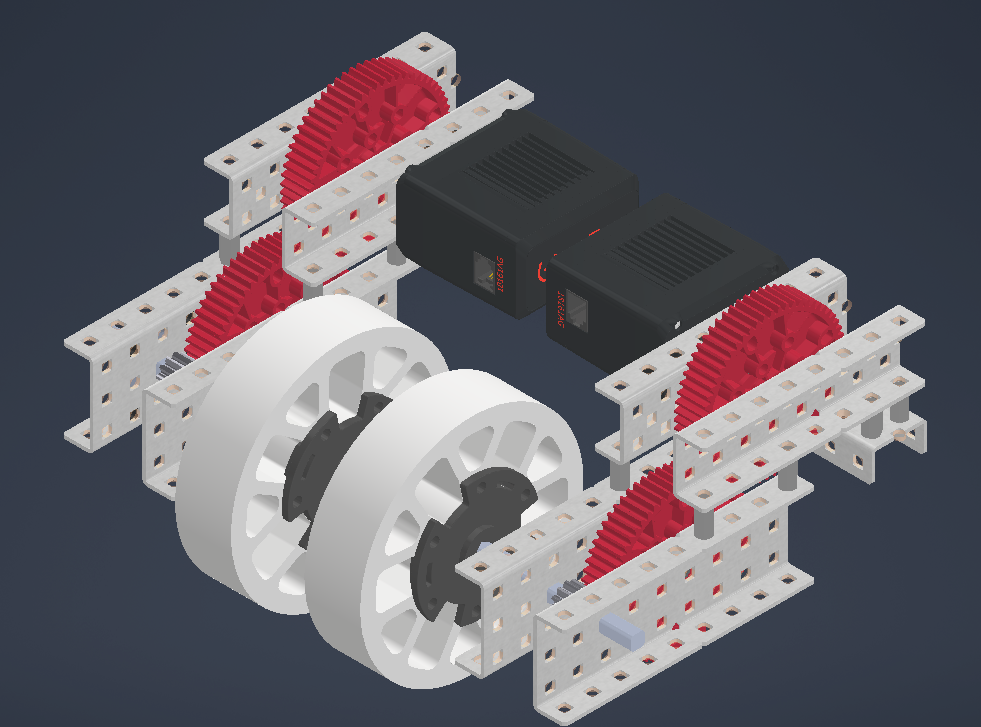
\includegraphics[width=0.52\linewidth]{images/15 cad/15Fly.PNG} \hfill  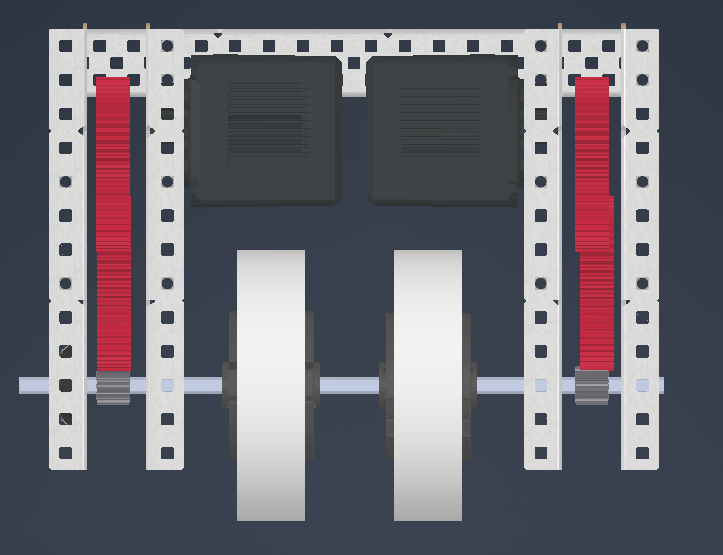
\includegraphics[width=0.5\linewidth]{images/15 cad/15Fly3.PNG} 
\end{figure}
\subsubsection{Testing}
\subsubsection{Problem:}
\par Building the flywheel CAD proved to have some challenges.  Upon first assembling the flywheel, we
noticed that had lots of friction issues
\subsubsection{Possible Soultions:}
\begin{itemize}
  \item Flywheel not square
  \item Spacing was off
  \item Bearing issues
\end{itemize}
\par Considering many sources of friction, we tested the flywheel wattage and recorded the following data:
\insertimage{images/15 tables/flywheel friction test.PNG}{0.85}
\pagebreak
\subsection{Competition Robot CAD}
This is the CAD that closely resembles the 15" competition robot
\insertimage{images/15 cad/15 Inch Robot.pdf}{.22}
\subsection{Fabricated Components}
Since there is not a vex part for everything, the team often turns to utilizing cad software
to create custom 3D printed parts. For the 15-inch robot, many of the printed parts are used to provide
structure and improve the stability. Some parts include:
\begin{itemize}
  \item Chassis Support Blocks
  \item Rear Chassis Intake Support Brackets
  \item Motor Stack Support Brackets
  \item Intake Brace
\end{itemize}
\section{Miscellaneous}
\subsection{Odometers}
A problem for the autonomous period for both skills and match play is how to accurately measure the 
distance the robot has traveled on the field. For Vex Spin Up, we designed our own odometry hubs for
both of our robots. However, during last year's competitions, problems arose due to the lack of structural integrity
our odometer pods had and their bulky size. This year, the team decided to:
\begin{itemize}
  \item Reduce the overall size of the hubs
  \item increase the durability of the prints
  \item increase the number of mounting positions 
\end{itemize}
These decisions were made so that being able to go over the barrier would not only be possible but also minimize
the risk of destruction when traversing over. In order to meet the listed criteria, a complete redesign was started
at the beginning of the year. The redesign was started due to a member of the club bringing to attention that Vex Pro offers 
two-inch omnidirectional wheels. Thus, the odometers could be reduced to an even more compact design. Our goal
was to incorporate the presented solutions into our final design. The only disadvantage we faced was trying
to create something that proved to be stronger while also being even smaller than last year's design.
The preferred time to have this completed was aimed at only taking three weeks, so that there would be two weeks 
of cadding and then one week of implementation and troubleshooting. However, this was not achieved due to the 
complexity of the redesign. The odometer design went through 4 iterations since the start of the year.

\begin{enumerate}
  \item Initial Iteration
  \begin{itemize}
      \item The first design was simply the same design as last year but created more compact so that it could be mounted in a tighter space. 
  \end{itemize}
  \item Second Iteration
  \begin{itemize}
      \item The second design incorporated the use of the two-inch omnidirectional Vex Pro wheels. This created an even more compact design than the first. The odometers were then printed with an increased infill to give them more strength. In addition, wider mounting brackets were installed that came with the purchase of the odometers.
  \end{itemize}
  \item Third Iteration
  \begin{itemize}
      \item The third design involved reprinting the odometers with a new support that provided more strength than the previous print. After this, the odometer mounting positions were rotated so that wire management would be easier.
  \end{itemize}
  \item Final Iteration
  \begin{itemize}
      \item The final design involved a fourth and final reprint. The previous support was removed in favor of a thicker support piece that was added to compensate for the overall thinness of the print.
  \end{itemize}
\end{enumerate}
There were not any more changes made to the design after the fourth iteration, but when constructing the odometers
we noticed that the axle holes did not come out correctly during the print due to overhang. Due to the need to begin odometry testing, 
we decided work with what we had and make the best of them. We decided to heat up the shaft that was to run through the holes and spin it through so that the axle could widen 
and smooth out the filament.
\insertimage{images/february/Odom_assembly.jpg}{0.1}

\section{24 Inch Design Selection}
This section will detail an in-depth overview of the 24-inch robot. It will discuss all integral design 
components as well as every subsystem and other aspects of the physical bot. Within this description will 
be detailed information regarding the overall design process, building methods, design choices, and 
difficult challenges the team faced while constructing their ideal robot for this year's Vex robotics season.
\subsection{Vision}
To effectively integrate professional software and methodology into our design and building process of a 24"x24"x24" robot. Our robot must 
be able to flawlessly integrate into, as well as, manipulate field elements of the 2023-2024 Vex Robotics: Over-Under Competition. In addition to 
meeting these criteria, our design has to fall within all technical rulings in order to stay legal. With the previously given parameters for size, being a 36" horizontal and limitless vertical expansion, the 24" robot must be able 
to do all that the 15" can and more. Here are some of the specific features the team would like for the robot:
\begin{itemize}
  \item Ability to manipulate triballs
  \item Efficient match-loading capabilities
  \item Ability to pick itself up for hanging points
  \item Clear under the elevation bar
  \item Capable of climbing over middle barrier
  \item Ability to hold and move triballs around
  \item Drive balance between speed and force 
\end{itemize}
With these goals for our 24" bot, we can match them up with subsystems that are comprised of VEX hardware and custom fabricated parts 
that are designed to complete these tasks as efficiently as possible. Here are the subsystems assigned to their individual goal:
\begin{center}
  \begin{tabular}{| c | c |}
    \hline
    \bf{Subsystem}      & \bf{Goal}                         \\
    \hline
    Wings               & Manipulate triballs                  \\
    \hline
    Intake              & Match-loading                \\
    \hline
    Endgame mechanism   & Picking the bot up               \\
    \hline
    Compact designs for subsystems          & Clear elevation bar                     \\
    \hline
    Skirt Wedge                             & Clearing middle barrier \\
    \hline
    Drivetrain                              & Balancing speed and torque                         \\
    \hline
  \end{tabular}
\end{center}
\subsection{Drivetrain}
\subsubsection{Problem Statement:}
We need to have a drive that is capable of generating enough torque to be powerful on the field, while also staying nimble in 
order to quickly interact with game elements.
\subsubsection{Solution Requirements:}
\begin{itemize}
  \item Must fit within a 24" x 24" x 24" cube at the beginning of the match
  \item At least 6 drive motors for torque capabilities
  \item Must comply with $<$VUR4$>$ for any fabricated parts used
\end{itemize}
\subsubsection{Drive type}
Referencing the list provided in the 15" drive section, the team working on the 24" robot decided that a tank drive would 
fit our criteria the best. A simple design matrix list is provided below to show what swayed our decision:
\insertmatrix{design-matrices/drive-iteration-1.tex}{First iteration drive train design matrix.}
\subsubsection{Design}
\par As the team collectively decided that a tank drive would best fit our criteria of having a great balance between maneuverability
and simplicity; they began construction. Below is the simplest rendition of the drive that the team had in mind. This design features a 6-motor, 257RPM, 6 wheel drive-train. 
We took inspiration from last year's 18" robot and implemented these ideas in a way that would cater to what we knew worked well, as well as what we believed would 
give us an advantage over this year's game. Below is the complete CAD drawing of the 2022-2023 Spin Up, 18" drive.
\insertimage{images/24cad/18WorldsBase.PNG}{0.75}
\par Learning from our mistakes in last year's competition, we knew that the drive had to be designed with rigidity and cohesive spacing in mind. 
This is why we designed 3D-printed chassis-blocks that would integrate in each of the four corners in the drive. These pieces would nearly perfectly align the 
holes of the outer and inner c-channels as well as provide structural support and set the perfect spacing for our wheels and gears to fit between.
Here is a detailed drawing of this piece with an example of how it mounts:
\insertimage{images/24cad/24_notebook_1.pdf}{0.3}
\subsubsection{Testing:}
Just like we the 15" robot, we tested the wattage of the drive and found that the left side was pulling
more watts than the right side. We then took the same test (found in the table below) and took the same steps
that were done with the 15". The results are listed in the table below:
\insertimage{images/24 tables/24 drivetrain test.PNG}{0.8}
\par After mounting these 4 pieces, the frame of the drive was essentially ready to have bearing flats installed. We use these to 
reduce friction between the low-strength shafts and the holes of the aluminum c-channels. The bearings also ensure that the shafts are aligned 
correctly to prevent binding between the gears and wheels that they run through. The next step in this process was to assemble the 4" omni-wheels and 84T high-strength gears. 
By connecting the two together, we save the headache of having to meticulously fit both the wheel and gear on a shaft with the perfect spacing. The assembly consists of these two components connected with screws and 
the minimum amount of spacing that keeps the rollers on the omni-wheels from contacting anything. We also figured out that a shaft collar could be placed in-between the gear and wheel, so that we could minimize the footprint that 
the drive-train has on the overall width of the robot. 
\par After the wheels were complete, we moved on to mounting the 36T gears that would be directly driven by our blue cartridge 600RPM motors. This would allow us to achieve a max RPM of 257. Additionally, we stacked our rear motors in order to conserve space for the front of the robot.
Once everything was cross-braced for stability, our drive for the 24" was complete:
\insertimage{images/24cad/Base.pdf}{0.2}
\subsection{Flywheel}
\subsubsection{Problem Statement:}
\par Create a consistent flywheel mechanism that shoots triballs consistently and at the correct height.
\subsubsection{Solution Requirements:}
\begin{itemize}
  \item must traverse under short barrier
  \item must fit within the 24" x 24" x 24" size constraint
  \item must be able to easily interact with game elements
\end{itemize}
\par Another integral subsystem of the 24" is the flywheel. We decided to design it before anything else on the bot once the drive was finished so that everything else would be made to fit around it.
We knew that the flywheel had to be elevated a fair distance above the chassis, so we utilized the c-channels that hold the stacked motor of the drive to build on. 
The most challenging aspect of designing the flywheel was not only condensing our space usage, but also creating something similar to a frame that we could continue to mount 
components on. Paying attention to this would help us a great deal in the future, when space for extra subsystems was not available. With this in mind, we mounted our motors diagonal in respect to the direction of where the actual high-strength shaft that would hold the flex-wheels is located. Finding the correct spacing for 
splining gears together at an odd angle proved to be challenging, yet allowed us to keep the design's simplicity. Directly driven by two 600 RPM blue cartridge motors were 60T high-strength gears. These gears were spliced one to one with another set that connected to a 12T pinion that would maximize the velocity our flywheel could achieve. This gear ratio created a maximum RPM value of 3,000, which would be more than enough to launch tri-balls across the field from our match-loading zone. 
Below is an isolated rendition of our flywheel, accompanied by a drawing depicting what it looks like mounted to the bot:
\insertimage{images/24cad/Flywheel.pdf}{0.2}
\insertimage{images/24cad/Base_Wing_Flywheel.pdf}{0.22}
\subsubsection{Testing:}
Just like how we tested the friction on the 15" flywheel, we tested it on the 24".
We noticed that at max speed it was not pulling a wattage we were happy with, so we took the same
approach, and were able to get close to same pulled wattage as the 15". The results are found in the table below:
\insertimage{images/24 tables/24 flywheel friction test.PNG}{0.8}
\subsection{Intake}
\subsubsection{Problem Statement:}
\par Create an intake mechanism that can retrieve match loads
\subsubsection{Solution Requirements:}
\begin{itemize}
  \item Intake must be able to reach over match load barrier
  \item Intake must start within 24" x 24" x 24" area at the start of the match
\end{itemize}
\par The next subsystem that operates directly tandem with the flywheel is the intake. By choosing a design that allows the intake of the robot to be mounted on a pivot point, we are 
able to conserve much more space by retracting it, while also increasing our reach by extending it as well. The team decided on 
running the intake off of a single 600RPM blue cartridge motor that drives a 30T sprocket that is chained to another 30T, creating a one-to-one gear ratio of 600RPM. The initial design of the 
intake support bars featured them as 1-by angle brackets that support another set of angle brackets that hold the motor assembly, along with the sprockets and support brace. The sprockets are tensioned with rubber bands, allowing triballs to make contact and be pulled in due to their elasticity. 
A rendition of the first intake iteration is provided below:
\insertimage{images/24cad/24_notebook_2.pdf}{0.2}
\par The 3D-printed cross-brace spanning across the intake is used in both old and new iterations. This piece 
acts as an effective substitute to an aluminum c-channel by cutting down on weight as well as providing a triangular brace, which reduces torsion forces that act upon the assembly. 
They integrate alignment pegs that are extruded out from the bottom of the component. With the addition of this piece, the intake is able to have less head weight so that retraction is not straining the motors with a large load. 
The CAD drawing for this piece is provided below: 
\insertimage{images/24cad/24_notebook_3.pdf}{0.2}
\par With the redesign of the intake, support bars were replaced with c-channels to increase structural stability at the cost of a small amount of added weight. The problem we faced with the previous design was that the 1-by aluminum angles were too 
flexible, having only two sides and being half the size of a c-channel. This caused them to buckle under pressure whenever a large force was imposed on the front of the intake. This deformation caused the intake to become inconsistent, thus 
demanding a redesign. Once the intake was operating properly, there was concern about the bands spanning between the front sprockets constantly being ripped off from contact with the goal. To fix this problem, we designed a component that would mount on the outside of the intake to essentially make contact with the goal just before the sprocket does.
CNC'd from Lexan, this piece allowed drivers to comfortably ram triballs into the goal without having to worry with damaging the intake. This would help to focus our attention to scoring and helps drivers to have more trust in the bot's structural integrity. 
A rendition of this component is provided below:
\insertimage{images/24cad/24_notebook_4.pdf}{0.2}

As you can see, this custom designed piece integrates with the front of the intake and mounts securely in order to relieve some of the force applied.
\subsubsection{Intake Retraction Mechanism}
\subsubsection{Problem Statement:}
\par Need to have a way to have the intake retract inside the robot and extend to be able 
to reach over the match load zone.
\subsubsection{Solution Requirements:}
\begin{itemize}
  \item intake needs to retract back towards the bot
  \item intake will need a hard stop to prevent overextension
\end{itemize}
\par Although the intake (static) would operate successfully, the team decided that both bots need to be adaptable to any situation. With this thought process, came the intake retraction mechanism. Despite its design being intended for match-loading, it 
\subsection{Intake Retraction Mechanism}
Although the intake (static) would operate successfully, the team decided that both bots need to be adaptable to any situation. With this thought process, came the intake retraction mechanism. Despite its design being intended for match-loading, it 
has many uses within a competitive setting. To begin describing this subsystem, its design allows for both driver-control and autonomous-mode to match-load triballs much more efficiently. One of the problems the 
team faced was shooting as many triballs across the field as possible. If the intake were static, the bot would have to, after shooting, move back and drive forward and extend the intake into the match-loading zone to shoot again. 
After brainstorming and prototyping, we came across a design that fixed this issue and more. The retraction mechanism includes a motor, positioned further toward the back of the bot, that operates a custom-printed component. This component is then connected to 
a static bar that stays parallel with the ground. The bar has a direct screw-joint connection with the rear support bar of the intake. This assembly is mirrored on the other side of the bot to ensure an even extension and retraction of the intake. 
With this mechanism integrated with the intake, we are able to keep the bot stationary while match-loading and simply retract the intake when another triball needs to be loaded in the zone. 
A rendition of the subsystem is provided below: 
\insertimage{images/24cad/24_notebook_5.pdf}{0.2}
As seen in the depiction, there is a 3D-printed arm that allows the control arm to pivot in a forward to backward motion. The red component is a squaring piece that aligns the assembly and 
keeps everything from flexing out of its intended position. These custom fabricated parts conserve the use of VEX hardware as well as space in the subsystem assembly. 
\subsection{Wings}
\subsubsection{Problem Statement:}
\par Design a wing mechanism towards the front of the robot capable of plowing triballs into goal
\subsubsection{Solution Requirements:}
\begin{itemize}
  \item fit on the side of the robot
  \item powered by double acting piston
  \item achieve maximum wingspan
\end{itemize} 
\par When approaching ways to push triballs into the goal, our first thought was pneumatics. These needed to be able to retract and deploy some sort of geometry that 
When approaching ways to push tri-balls into the goal, our first thought was pneumatics. These needed to be able to retract and deploy some sort of geometry that 
avoids concavity. This means that, while moving, our robot cannot have more than one triball moving with it, indicating double possession. To solve this problem, we decided on a mechanism known as wings, that would deploy 
perpendicular to the left and right sides of the robot. This way, we could avoid being called for possessing 2 balls, while also having an upper-hand with triball manipulation. These "wings" would increase our horizontal span of the robot to right under the maximum amount of 36 inches.
This width is quite large to have deployed all at one time, so we knew that both double acting pistons had to be wired with separate actuators. Doing this also helps with building air pressure on each piston, so they have less give when pushed against. Mounting 
the double acting piston was the most challenging aspect of this assembly due to the constraints we had regarding possession. This meant that the wings could never over-center while manipulating triballs. 
Rotating joints were the key to making this concept a working reality. The piston itself, as well as the bar holding the wings, both had to be on a joint with bearings to ensure a smooth rotation. 
Now, as far as what would actually contact the balls, we designed a piece to be CNC'd out of Lexan that would hit the triballs low enough to wedge above the low barriers. We also had to design a transitional extrusion from where the bar was located, to a very 
rigid location, such as the chassis. A CAD drawing for this subsystem and its components are provided below:
\insertimage{images/24cad/24_notebook_6.pdf}{0.2}
In the drawing given, the triangular component is designed to be 3D-printed, where it would transfer the force applied to the wings onto the chassis. This helps us keep our fragile pneumatics from being deformed and possibly 
undergoing catastrophic failure during a match. The larger Lexan piece is designed so that they wedge triballs upward, allowing the bot to hit them with enough force to transfer them over the middle barrier. With all these components combined into an assembly, we 
have a great way for moving triballs into goals.
\subsection{Testing:}
\par Seeing that we had more space to work with on mounting the pistons on the 24", we wanted 
to mount them parallel with the chassis create a more compact mounting position. However, we
ran in to the issue of this mounting position not providing enough of an angle to deploy the wings.
As a result, we ran a moved the mounting position of the piston closer into the center of the robot to create
a better angle. We recorded these results in the table below:
\insertimage{images/24 tables/wing mounting test.PNG}{0.8} 
\subsubsection{Endgame Mechanism}
\par The final subsystem to be designed and constructed on the bot, is the endgame assembly. Given a larger area to build with, the 24-inch weighs in at approximately 25 pounds. This makes it 
have a great way for moving triballs into goals. 
\subsection{Endgame Mechanism}
The final subsystem to be designed and constructed on the bot, is the endgame assembly. Given a larger area to build with, the 24-inch weighs in at approximately 25 pounds. This makes it 
very hard to achieve a decent hang in the last moments of a match. However, weight is not our only problem; the only space left on the robot at this point was secluded to the rear end, away from its center of mass.
Constructing an endgame mechanism at this point would require even more torque power to compensate for an uneven distribution of weight being pulled. To accommodate for this, the final design we chose uses the most amount of torque 
possible from 2 red cartridge motors, while having enough time to deploy the mechanism. Our team decided it would be best for the first iteration of our endgame to try and achieve a low hang of "A," or "B" tier. 
This would mean that the robot would have to pick up its entire weight and hold its position even when power is disconnected. Knowing this, we knew that 
an arm lift was possible, but the problem still remained of how we could keep the bot from falling down and contacting the field due to its immense weight. The design started with two towers; one on each side near the back of the bot. 
Each tower has a red VEX motor driving a 12T pinion, that spins an 84T gear. These gears are both connected by a single high-strength shaft to equalize the torque on both sides. 
Attached to the 84T gears are c-channels that have stand-offs positioned to make contact with the low bar and lock the bot in place. The mechanism begins folded down in order to conserve space for the robot to pass under the low bar freely during match-play. 
Whenever it is time to hang, though, the bot extends the arms up and pulls them down, thus pulling the robot up off of the ground and closer to the bar. This action works well, but there needs to be something to lock the gears in place and without power, it has to be something mechanical. 
This is where our design for a pneumatic ratcheting mechanism comes into play. With our small, double-acting pistons, we can deploy them in-between the 84T gear and 12T pinion to keep the bot from falling. 
A rendition of this assembly is provided below:
\insertimage{images/24cad/24_notebook_7.pdf}{0.2}
\subsection{Complete CAD Rendition}
\insertimage{images/24cad/24Assembly_ATUM.pdf}{0.3}
\section{Fabricated Components}
With every subsystem of the 24" and 15" robot, there are many instances where a fabricated part works much better than that of VEX hardware. 
As the robots become more sophisticated, it is important to find these issues where we may be using too complex of a mechanism and simplify it by fabricating our own 
component. This is one of our major goals with these bots, being simplifying as much as we can at no cost to performance. What we have found in the past is that the simpler a mechanism is, the more likely it will be to operate without error. 
There are many components like this that we have fabricated. From 3D-printing to CNC, we can use these methods to simplify and improve our bot's design. 
Most of our mechanical-oriented fabricated parts are made with one of our Raise3D, 3D-printers. We use different plastic filaments for various applications, such as PLA and ABS.
Depending on how vital this piece is to the structural aspect of the bots, we will adjust their infill density to either something more empty, to a solid object. Doing so can help us save on time as well on material used. 
Our CNC machine is used mostly for objects that are 2D oriented and only require a thin amount of material. This is due to the fact that a CNC is meant more for working with cut-outs and thin material. For 
each of our fabricated parts listed, there is an indicator of which bot they are made for and what method/material was used in the final design process. Here are our fabricated parts:
\insertimage{images/fabricated/15 Skirt Reinforcement.pdf}{0.3}
This component is used as a reinforcement for the 15" skirt when the bot makes contact with the middle barrier in order to climb over.
\insertimage{images/fabricated/15_RearWing.pdf}{0.3}
This Lexan piece is used on the 15" to deploy and move triballs.
\insertimage{images/fabricated/Arm.pdf}{0.3}
This component is used on both bots and allows the intake to be extended and retracted by a motor. The shaft runs through the square insert and the screw joint is mounted in the circular hole.
\insertimage{images/fabricated/15 Skirt.pdf}{0.3} 
This CNC'd component is used to protect the chassis from anything that would come in contact with the drive-train. It also protects the gears from grinding when passing 
over the middle barrier. 
\insertimage{images/fabricated/RearChassisBlock.pdf}{0.3}
As previously shown, this 3D-Print aligns the chassis, while also enforcing every corner for each bot. 
\insertimage{images/fabricated/RLBrace - Copy.pdf}{0.3}
This 3D-Printed piece is used between both bots to align the assembly of the intakes as well as brace between them. This allows the intake to extend and retract 
evenly and avoid binding up in operation.
\insertimage{images/fabricated/Standoff Blocks.pdf}{0.3}
This 3D-printed component provides support to the rear end of the 15" flywheel as well as other assemblies that are mounted around it. It features alignment pegs, with two holes for screws to go through and tighten the component down on both sides.
\insertimage{images/fabricated/24_Skirt.pdf}{0.3} 
Similar to the 15" skirt, this 3D-Printed object keeps the drivetrain of the bot protected. It also features a sled-like design at each end to help reinforce 
the Lexan pieces that allow the 24" to go over the barrier. 
\insertimage{images/fabricated/24_SkirtBrace.pdf}{0.3}
As just mentioned, this sled piece is CNC'd out of Lexan, making it able to take the force of the bot going over the middle barrier. This joins together with the 24" skirt to make an 
even stronger and more durable piece to contact the barrier. 
\insertimage{images/fabricated/24_Wing.pdf}{0.3}
This CNC'd Lexan Wing is used to puch triballs around the field, while also having enough rigidity to wedge them into the goals. This allows us to effectively score without having to manipulating a c-channel to this geometry.
\insertimage{images/fabricated/Intake_Controlmtr_brace.pdf}{0.3}
This 3D-Printed component wraps around the geometry of the intake retraction mechanism and aligns everything to the correct spacing. Its low profile keeps it out of the way of other moving parts, while 
supporting this important subsystem of the robot.
\insertimage{images/fabricated/Wing_Brace.pdf}{0.3}
This wing brace helps to transfer force from the wings to the chassis - a more rigid surface. Without this, our wings would surely be deformed after a few uses.
\insertimage{images/fabricated/intake_skirt.pdf}{0.3}
This CNC'd Lexan piece guards the front intake sprockets, allowing the bot to ram against the goal with no ramifications. This helps drivers to run at faster speeds without 
worrying about damaging one of the more sensitive subsystems of the robot. 
\pagebreak
\addtocontents{toc}{\setcounter{tocdepth}{1}}
\section{15" Log}
\subsection{10/04/2023}
Juan, Hunter, and Preston began to build the wheel assemblies.

\subsection{10/13/2023}
Juan and Hunter began to assemble the chassis and the drivetrain. They then installed
the wheel assemblies, and completed the drivetrain. This was done on only one side
in order to find the ideal spacing. After the appropriate spacing was agreed upon,
they squared the chassis off and installed a few motors. At this time it is important to note that they
were missing the 3D prints that are located in the 15" cad and were using last year's motor stack
support prints which were found to work out better than what was in the cad.

\subsection{10/19/2023}
Juan and Hunter replicated the drivetrain onto the other side of the chassis. They then began to
look and find the ideal spacing so that both sides would have the least amount of friction. Eventually,
the chassis was completed, and the chassis was squared off. At this time the robot is still missing the
intended 3D prints located on the cad. They then installed the motor covers for future reference since
they were still missing two blue motors. After the completion of the chassis, Juan began to cad
the wings and the intake.
\insertimage{images/october/completed15chassis.jpg}{0.1}

\subsection{10/28/2023}
Before working on the intake, Hunter and Juan installed the front and rear chassis support blocks
to further stabilize the chassis. After this, they began to work on the first iteration of the wing assembly.
They aimed at using the cad that was created, however, it was soon found out that they would need to deviate
from the cad and change to a 3 by c channel to house the piston. This was done on only one side and is still
in the process of being finalized. They then proceeded to move on to building the intake. The first design
of the intake was directly drove with a 200rpm green motor. While building the intake, it was decided that the
cad was not going to work as expected and changes were made. They then proceeded to work on designing the
intake retraction mechanism. The first iteration came with using a 200rpm motor, but this did not provide
the necessary torque to retract, thus Juan began to cad iteration 2.
\insertimage{images/october/first iteration of intake.jpg}{0.1}

\subsection{11/01/2023}
Juan, Hunter, and Collin installed the 3D printed intake brace.

\subsection{11/02/2023}
Juan and Hunter built the second iteration of the intake retraction arm. They also began tuning the intake
and retraction arm extension. Through the tuning of the intake, it was decided to add a blue motor in place of
the green motor so that the triballs would intake more efficiently.

\subsection{11/09/2023}
After long consideration, it was decided the retraction mechanism was taking up too much space. Hunter and
Juan decided that iteration 2 needed to be slid back on the robot to allow for more space of future subsystems.
Everything else regarding the intake and the way it retracted remained the same. Also, the team decided with
this new allocated space a flywheel would be able to fit inside the robot and be the way the 15" manipulates
the triball.

\insertimage{images/november/final iteration of retraction mech.jpg}{0.1}

\subsection{11/10/2023}
Juan slid back the other side of the retraction mechanism and began to prototype a 3000rpm flex wheel flywheel
and how it could be incorporated into the robot. After seeing that the design had potential, Juan began to
cad the flywheel.

\subsection{11/16/2023}
Juan and Hunter installed new 3D printed intake supports blocks for the rear chassis that
provided both aesthetic and structure for the robot. They also noticed that the retraction arm motors
needed to be flipped in order to provide enough space for the flywheel assembly. The flywheel assembly was
then installed. At this time, another motor is still needed to power the flywheel, and they plan on switching
to regular high strength bearing flats instead of ball bearings.

\insertimage{images/november/top view of flywheel.jpg}{0.1}
\insertimage{images/november/sideview with intake extension.jpg}{0.1}

\subsubsection{11/23/2023 - 1/18/2024}
The team did not hold meetings or work on the robot due to the holidays.

\subsection{1/19/2024}
Upon returning from the break, Juan and Hunter installed the second motor for the flywheel and began testing to 
determine what was working and what was not. 

\subsection{1/21/2024}
Hunter and Juan mounted the brain and the battery and began to start routing wires on the robot. This was done 
to make flywheel testing easier. They experimented with what would have the best compression and allow the triballs 
to shoot consistently. 

\subsection{1/25/2024}
Juan, Hunter, and Braden continued flywheel testing. Braden programmed the flywheel toggle onto the controller for easier 
testing and began to play around with various rpms. After testing, they noticed that the flywheel's movement 
made the robot unstable, so they added additional rear bracing.

\insertimage{images/January/flywheel bracing.jpg}{0.1}

\subsection{1/26/2024}
The team was able to order some more blue cartridges so Hunter and Juan added the 5th and 6th drive motors which then
allowed them to incorporate the motor stacks from last year's robot used at Worlds.

\insertimage{images/January/boxed motor stack.jpg}{0.3}

\subsection{1/27/2024}
Juan began to practice ramming in triballs and the team realized that the chassis was beginning to cave in. Thus, they
decided to brace the chassis with standoff that run underneath the robot. Hunter and Juan also realized that the CAD wings
were not going to be able to work due to the 15" size constraint. They also continued tuning the flywheel.

\subsection{1/28/2024}
Seeing that the original wing design was not going to be feasible, Juan and Hunter began to prototype drop down wings
since the only way to make the cad design work would require a complete rebuild of the chassis. They decided that the
wings would be powered by two double-acting pistons and started looking at how they could be oriented on the robot.

\subsection{2/1/2024}
After prototyping, Juan went back to the cad and began looking at what might be the most reasonable way to mount the wings.
He was able to discover a more robust mounting system that would keep the robot in size and provide the wings with structural
integrity. The two of them then installed the new wing mechanism onto the robot.

\insertimage{images/february/first iteration of wings.jpg}{0.1}

\subsection{2/2/2024}
Since the new wing design looked promising, Juan mounted the air tanks on the robot so that they could be tested properly.
While testing, Juan noticed that the wing's integrity could be compromised if they were hit head on, so he braced them 
with a standoff collar joint mechanism.

\insertimage{images/february/braced wing and air tank.jpg}{0.1}

\subsection{2/3/2024}
While testing the wings, Juan and Hunter noticed that the pistons connected to the c-channel were beginning to bend.
They deduced this was due to the force of the stroke being applied when the pistons were activated. They decided to swap
out the SMC branded pistons for HLQD branded pistons since the internal piston shaft was stronger, and offered a better way 
to orient the pistons. However, the wings were still not deploying properly, so they added springs and rubber bands to help
the pistons have a more consistent stroke. The original wing design system was then removed since it was no longer needed.
Hunter and Juan also added additional support to reduce chassis torsion. The standoff bracing that was added also acted as a 
hard-stop for the intake retraction arms. This made the intake arms spin only in a semicircle and force it to stop at the
same spot every time.

\subsection{2/6/2024}
The team builders dyed the green intake sprockets black to add more of an aesthetic feature to the robots. This process
was rather simple and was done by boiling water, acetone, and black dye. The sprockets were then placed into the mixture
for a couple of minutes until the black dye had completely soaked into the gears.

\insertimage{images/february/real deal black sprockets.jpg}{0.1}



\subsection{2/7/2024}
Hunter and Juan replaced the green intake sprockets with the ones that the team dyed black. They also replaced the gears
that powered the intake arms with a 3d printed cam shaped PLA piece that mimicked the geometry of the 60 tooth gear that
was originally there. In addition, they replaced the red 3d printed intake brace with one that was black to make it look
more appealing. The team also began to mess around with the LED RGB strips and got them to work through the Vex brain. 
Juan also installed a 3d printed plate piece that covered the flywheel motors to make the robot look even nicer. 

\insertimage{images/february/rgb strips working.jpg}{0.1}
\insertimage{images/february/side view with plate.jpg}{0.1}

\subsection{2/8/2024}
Hunter and Juan mounted the license plates, wrapped the air tanks and pistons in a carbon fiber wrap, and the barrier ramps
that were in the CAD file were mounted. However, the compact nature of the 15" robot  affected the match loading capability 
of the robot. The 1/4" difference of where these ramps were placed drastically reduced the efficiency of the flywheel.
Luckily, the chassis was designed to be symmetrical, and the ramps were moved to the back of the robot. Unfortunately, the
robot was now out of size. So Juan and Hunter moved the intake hard stop had to be moved further in, so the air tanks could 
also be moved in as well. They also begin looking into potential IMU mounting positions. 

\subsection{2/9/2024}
In order to give a robot a unique finish, the team decided to anodize easily removable hardware or subsystems of the robot.
Most of these parts needed to be rebuilt into more competition ready variants, so they were going to be replaced anyway. 
Juan and Hunter disassembled these components and laid them out for an easier rebuild. The following parts were removed:

\begin{itemize}
    \item intake mechanism
    \item wings
    \item outer chassis components
    \item intake retraction bearings
    \item wing piston plate
    \item license plate mounting hardware
\end{itemize}

These parts were then cleaned thoroughly and went under a multi-stage anodization process. The removed parts
were scrubbed with dish soap, sprayed and scrubbed with a degreaser, and then rinsed off with distilled water.

\insertimage{images/february/removed c channels for anodize.jpg}{0.1}
\insertimage{images/february/15 anodize intake layout.jpg}{0.1}

\subsection{2/10/2024}
The next day, Juan, Hunter, Braden, and Collin started the next steps of the anodization process. 
Since the robot was taken apart, Juan and Hunter installed the IMUs in a suitable location
and mounted the GPS sensor. While the anodization process took many hours and the rebuild seemed to take even longer,
the team was happy with the results and how the robots turned out. 

\insertimage{images/february/anodize first step.jpg}{0.1}
\insertimage{images/february/anodize last step.jpg}{0.1}
\insertimage{images/february/anodized complete 15.jpg}{0.1}

\subsection{2/11/2024}
On this day, Hunter and Juan cnc'd the skirts out of ABS and mounted them and installed the odometers. Juan designed
an additional piece that was to be added to the wings so that they could push triballs more effectively. The team
was then donated a sheet of Lexan. Thus, the Juan and Hunter decided to cnc the pieces for the wings out of Lexan 
rather than ABS to provide more durability over time.

\insertimage{images/february/cnc skirts.jpg}{0.1}

\subsection{2/12/2024}
Since Braden wanted to create a macro that could be used for match loading, Hunter mounted the distance sensors inside the
intake of the robot. This would allow the robot to detect when triballs were placed in front of it and would know when it
could extend and retract with the press of a button. Juan then mounted a port expander at the back of the robot and cnc'd 
the aluminum ATUM plate. While this was being done, the team decided to run a couple of skills matches before leaving
the lab. Due to an extensive run time, the right intake bar snapped where it is connected to the retraction linkage.

\subsection{2/13/2024}
Everett replaced the snapped intake bar and then later that evening Juan and Hunter began working on more flywheel tuning.
While doing this, they realized that the flywheel needed to be spaced further apart to account for intake error. Rebuilding 
the flywheel did help keep the triballs straight but, in turn, reduced the compression and made the triballs not be able
to shoot over the barrier. They also reprinted the plate piece and added a piece of Lexan on top of it so the RGB lighting
could shine through the aluminum ATUM plate.

\insertimage{images/february/real deal atum.jpg}{0.1}

\subsection{2/14/2024}
Juan, Hunter, Preston and Everett worked on tuning the intake for skills with Braden and Darius and also practiced
match loading. While testing, the leftside intake bar snapped and the builders made the decision to replace both sides 
that snapped with c-channels.

\insertimage{images/february/snapped intake arm.jpg}{0.1}

\subsection{2/16/2024}
Braden and Chris continued tuning and noticed that the flywheel was not spinning properly. Upon inspection, they
found that the versa hubs were worn out due to friction caused by a cracked shaft collar. The versa hub were then
reprinted with ABS instead of PLA and were then replaced. After replacing them, Juan and Hunter continued to tune the
flywheel with Braden.

\subsection{2/17/2024}
Juan and Hunter helped Braden and Darius tune the flywheel for a few hours. This included trying out varying rpms
with different levels of intake extension and compression.



\section{24" Log}
\subsection{10/2/2023}
In today's meeting, Collin, Chris, and Payton worked together to begin assembly of the 24" bot in reference
to the CAD file. They put together the 6 wheels and prepared every gear with its own shaft, collars, and teflon washers. Afterwards, they put together
the basic frame of the robot, consisting of the inner gearbox c-channel, along with cross-bracing to keep everything together.
Eventually, they attached 4 motors of the drivetrain and put together the outer c-channel for the gearbox, which would accomodate for a stacked rear motor in order to save space.
Now that the general frame of the robot was built, they are ending the meeting with putting together last minute tweaks regarding spacing of the wheels and moving their attention to assembling the drivetrain.
\subsection{10/3/2023}
Collin and Chris worked on adjusting the spacing of the gear-train so that the motors would have less of a load
with a lower amount of friction between gears. Then, they began to finish the cross-bracing between both sides of the robot to ensure
rigidity of the entire assembly. This allowed them to worry less on the drive binding up, while also making the frame of the bot much more stable.

\subsection{10/4/2023}
With the frame of the 24" bot assembled, Collin came in and placed the appropriate
gears and wheels, forming a drivetrain. He added bearings to the inner and outer c-channels of the gearbox and made sure that
every gear was meshing properly in order to prevent binding. Once he found the proper spacing and technique in order to keep
every gear and wheel perfectly aligned, he repeated this for the other side of the robot. Now that the
bot is driveable, they will begin putting their efforts into different subsystems of the assembly. Refer to \ref{fig:24_chassis}.
\begin{figure}
    \centering
    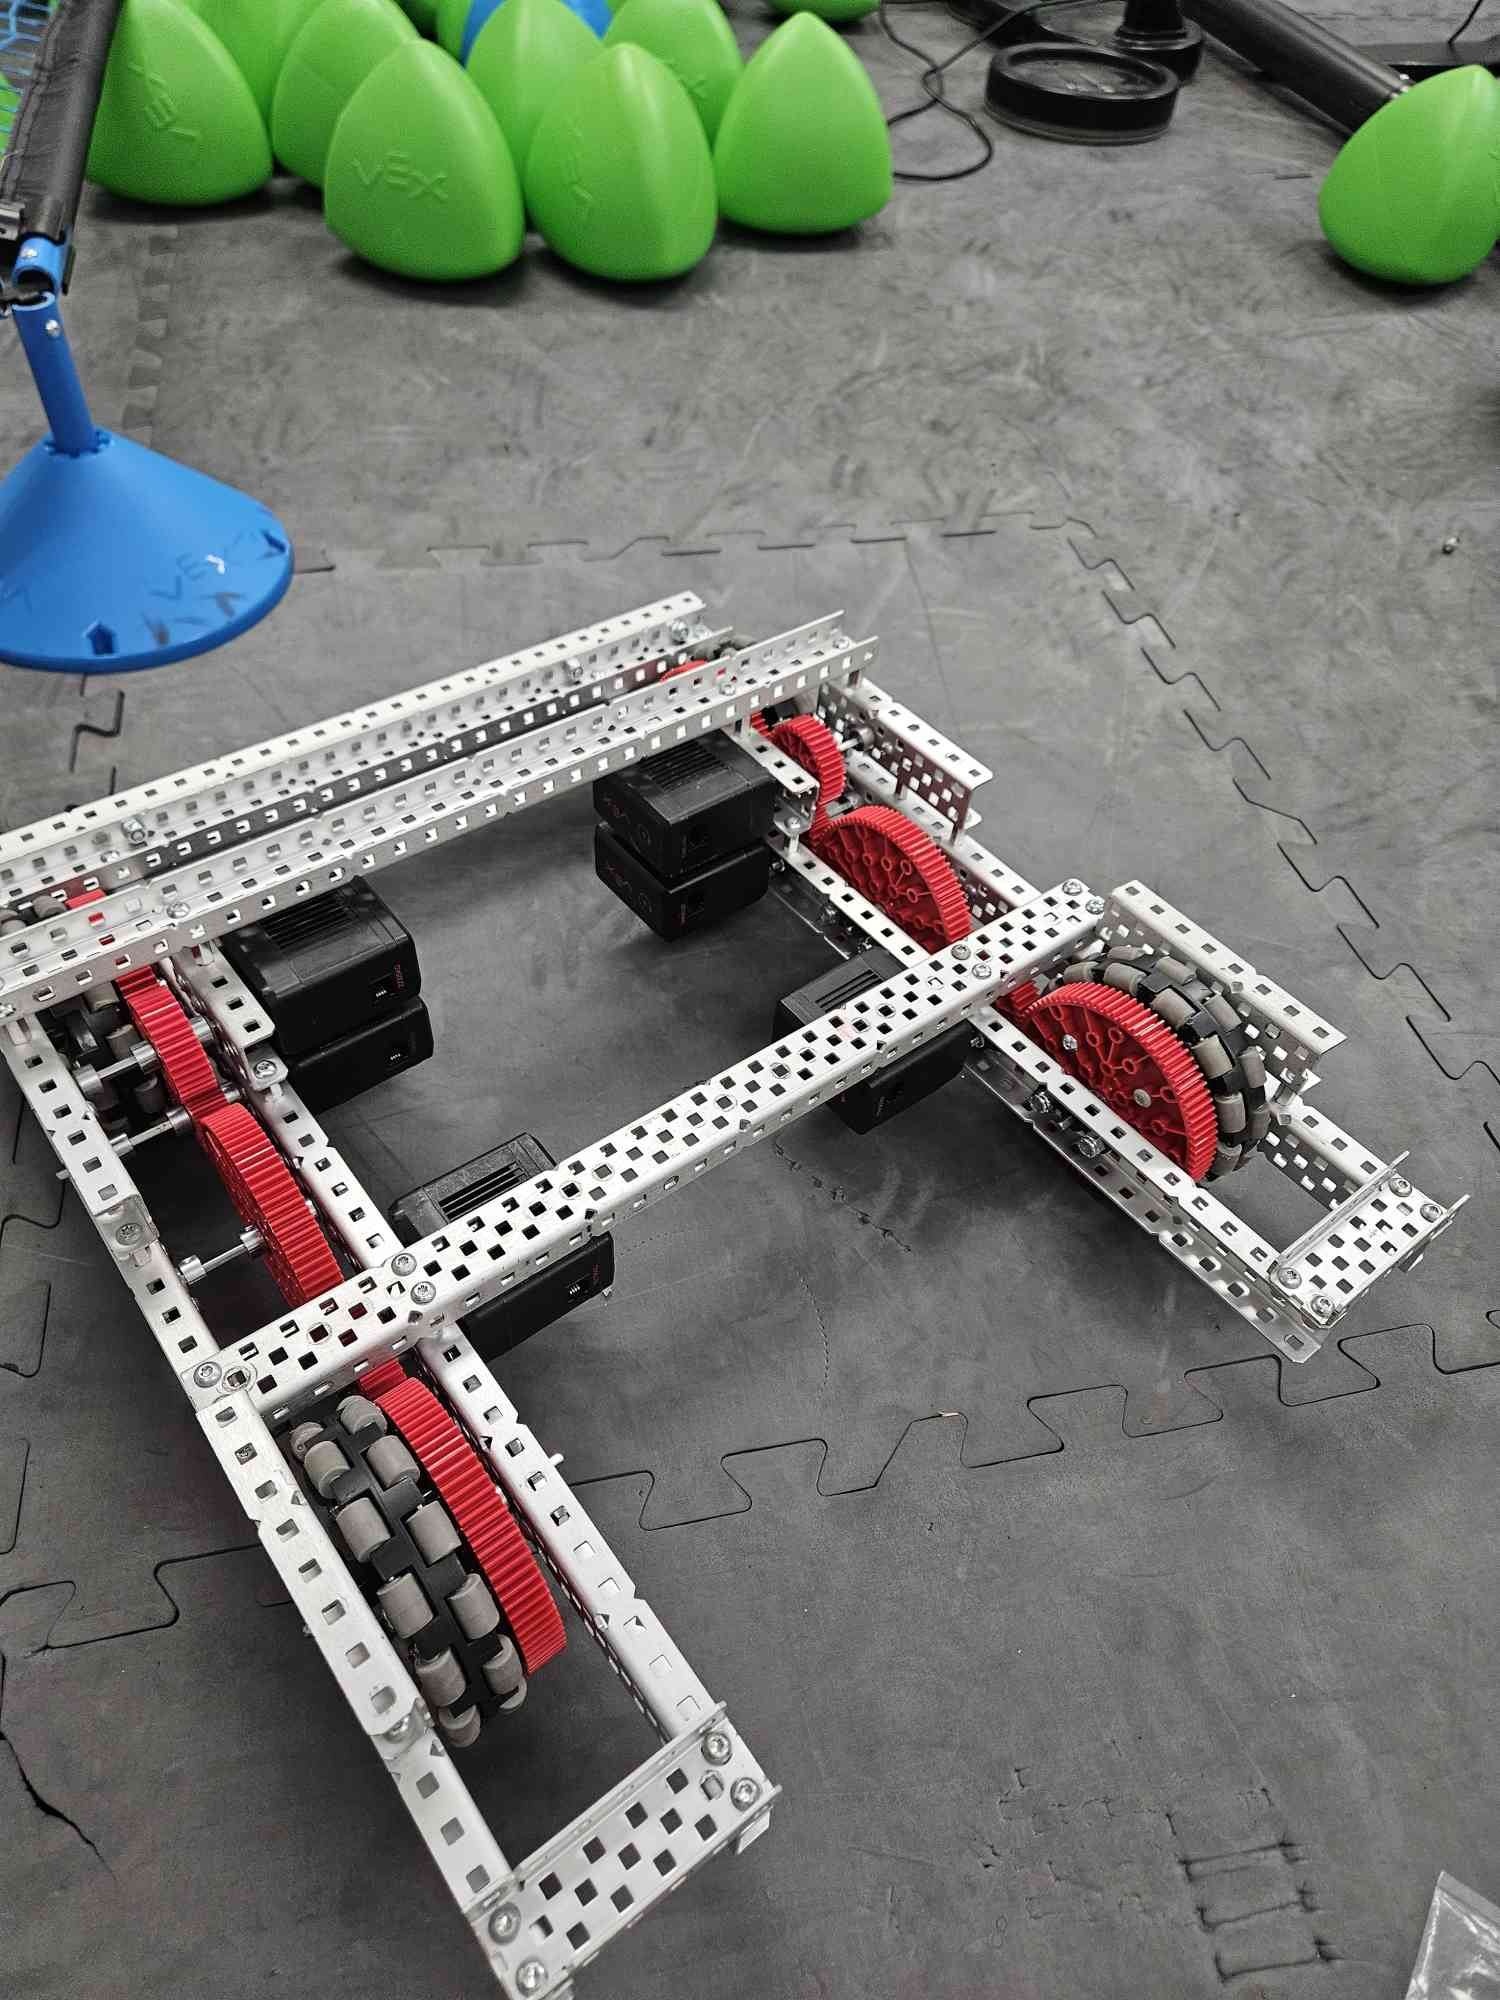
\includegraphics[width=0.5\linewidth]{images/october/24_chassis.jpg}
    \caption{The 24" chassis as of 10/4/2023.}
    \label{fig:24_chassis}
\end{figure}
\subsection{10/5/2023}
With what they had built now, it was time for testing the subsystems and perfecting small imperfections with their performance. Collin and Ryan worked on a drive motor and found it to be pulling too many watts, thus needing replacement. Then, Chris added a triangle brace comprised of standoffs to the outer piece of the intake. With the current edition of the CAD built, Collin began to design more cross-bracing and custom 3D printed pieces to keep the
intake control assembly aligned. He also updated the wing and skirt design in order to prevent possession calls of tri-balls.
\subsection{10/7/2023}
After everything with the drive train was wrapped up, there was nothing left on the CAD to build, so Collin began
to design a wing mechanism.
\subsection{10/9/2023}
As juan developed a way to retract and extend the intake assembly, Collin came in and replicated what he designed onto the 24".
This allowed the bot the ability to reach and intake tri-balls from the loading zone, while also retracting in order to stay within size constraints.
\insertimage{images/october/Intake_controller.jpg}{0.2}
\subsection{10/13/2023}
While the CAD was being worked on, Everett and Preston added another intake controller to the other side of the bot.
They did this so that the intake would retract evenly and not bind up as it would be used a great deal especially during autonomous. They also figured out that the speed the intake
moves at was far too slow. In order to safe space from forming a gear ratio, they decided to replace the green motor cartriges to blue, which run at a faster RPM.

\subsection{10/16/2023}
In the bot's current state, it is now time to begin testing designs for a flywheel. Ryan, Preston, and Everett worked on a design iteration that would test an elevated flywheel that makes contact with the top of tri-balls. Collin conceptualized a design that preserves space, in which the flywheel assembly is closer to the chassis, possibly allowing the 24
to pass under the low-bar of the field.
\insertimage{images/october/Flywheel_concept.jpg}{0.2}
\subsection{10/19/2023}
Today, Chris, Collin, and Payton began assembly of different subsystems of the robot. They found the correct sizing for the intake that would stay within 24" and critiqued the design from the CAD.
Collin also started testing different designs of the wing retraction mechanism. More bracing and support for these subsystems were added in order to keep building upwards for an intake control motor. Once the intake, wing mechanism, and intake control motor were completed, they began going over possible designs for a flywheel that would shoot the tri-balls across the field.

\subsection{10/28/2023}
Juan had already conceptualized a flywheel assembly by building on top of the intake control mechanism, so Collin adapted this design and made it cater to the larger bot's size. Later, Chris came and finished the job on the 
flywheel assembly after Collin had added c-channels in the correct position. Shortly after, the flywheel was built and they began to program the motors in the code to begin speed testing.
\insertimage{images/october/Flywheel_finished.jpg}{0.2}
\subsection{11/01/2023}
After a break to tend to studies, Collin and Chris came back and mirrored the intake control mechanism to the other side of the chassis. Without adequate bracing for the outer hub that holds the motor shaft, Collin went to design a piece to be 3D printed in inventor that would provide bracing and help align the tower in which the motor was mounted.
\subsection{11/02/2023}
The next day, Chris and Collin looked to tuning the intake of the robot and decided along with Juan and Hunter that a blue cartridge was better for the motor. This would help to intake tri-balls faster and more efficiently.
\subsection{11/09/2023}
After noticing a considerable lack of power with the intake, Collin and Chris concluded that is was most likely due to the high-strength shaft creating friction. They experimented with different ways to mount the banded sprockets
that would contact the tri-balls, including screw-joints and a low-strength shaft running through them. Ultimately, it was decided that returning to the high-strength shaft would be the best course of action, but they had to 
locate where the majority of friction was coming from.
\subsection{11/10/2023}
Chris and Collin eventually decided to change the mount for the high-strength shaft and bearings to reduce friction. The intake was now able to match-load quite well, although match-play would hold more problems that would need to be solved later on.
\insertimage{images/november/Intake_old.jpg}{0.1}
\subsection{11/16/2023}
After a short break, Braden had given us variable speed controls for the flywheel that we could test along with adding controller binds for the intake control mechanism. Collin began to work more with the pneumatic wings in which he 
decided there would need to be a lot more bracing in order to avoid deformation, knowing that a lot of force would be acting on this subsystem.
He then went on to CAD a 3D printable brace that would extend from the wing mounts to the chassis, ensuring that the force would be more evenly dispersed.
\subsection{1/19/2024}
Following Christmas break, the team got back together and bought more blue cartridges, so that we
 could put them in place for the green cartridges in the flywheel assembly, so that we could run the flywheel at higher RPM's, allowing us to shoot tri-balls farther.
\subsection{1/21/2024}
Today, in interest of saving space and cable management of the robot, Chris re-routed all motor cables to a new brain location, 
along with mounting the battery in a safer location. This way, we could minimize the space we were using as the bot is becoming more dense with further building.
\subsection{1/28/2024}
Ryan used the CNC machine to cut out the CAD renditions of the wings and skirt for the bot. Collin got these and mounted them to the wing bar and realized that the force it takes to prop
 the bot on the middle barrier was far too much for regular 1/8" ABS to handle. Aside from this, though, Collin did more work on mounting pneumatic actuators and running the tubing that would supply air to the double-acting pistons for the wings. This brought on a redesign for the skirt, along with the wing piece. Collin designed something more 
 similar to a sled that would lift the bot over the barrier as it runs into it. Afterwards, more tuning was done to the flywheel, such as adding rubber heads that are spaced to where they 
 make contact to the tri-balls before hitting the flywheel. This was done in order to create more compression on the balls as they shoot out from the bot. 
\insertimage{images/february/Sled.jpg}{0.2}
 \subsection{2/1/2024}
Following up on the match-loading capabilities of the intake, Chris began testing with cross-braces on the 
front end of the bot so that tri-balls would be held with more compression as they are brought up to the flywheel. In addition to this, a brace that was previously designed was 3D-printed that spanned between both sides of the intake.
Collin also began constructing a new mounting position and brackets for the wing assembly. This would conserve space and allow the pistons to have more leverage when deploying.  
\insertimage{images/february/New_pistons.jpg}{0.2}
\subsection{2/2/2024}
With a little extra time, Braden, Juan, Hunter, and Collin decided to follow through with an idea from last year regarding anodizing aluminum.
 They took apart a few external pieces of each bot and took them to another lab in order to strip them and dye them black to enhance aesthetics. 
\subsection{2/5/2024}
Finishing the renditions of the bot's skirt, the team decided it would be best to use 1/16" ABS for the skirt and make the sled pieces out of thicker 1/4" lexan. Collin also added more of these sled 
pieces on the rear end of the bot so that it would be able to maneuver itself over the middle barrier in any orientation to make it easier on the drivers. He also designed a guard that would be made out of lexan that would cover the radius of the intake
 sprockets so that the intake could essentially ram against the goal when it was pushing tri-balls to score. This would ensure that no damage would be done to fields and also 
 that our chain linkage within the intake wouldn't be in any danger of breaking loose.
\insertimage{images/february/Skirt_complete.jpg}{0.2}
 \subsection{2/7/2024}
 With most of the subsystems finished, it was time to put more effort toward pneumatics and more cable routing.
 Collin began by mounting the air tanks under the chassis of the robot so that they would be out of the way, while also keeping a lower center of gravity for the robot.
 Additional pneumatic fittings and actuators were also mounted securely to ensure that nothing would be getting pulled loose and disconnected. Ryan continued by mounting sensors on the robot, including 3 IMU's above the air tank
, so Braden could use the data they output for his programming with autonomous. Distance sensors were also added in the front of the bot so that his program could tell whether or not a tri-ball was being matchloaded by 
measuring the distance between the sensor and the wall and that value being shorter whenever a ball is placed.
 \insertimage{images/february/Air_tank.jpg}{0.2}
 \subsection{2/9/2024}
 In order to let Braden continuing testing with his autonomous program, Collin and Chris conceptualized where to mount odometers on the robot so that they would be out of the way of any moving parts, while also being able to pass over the middle barrier. 
 This year's design for the odometers were much smaller, so we could fit them in hard-to-reach spaces. After a few test-mounts were made, the team found out that the odometers had to be placed at a certain angle, so only the wheel would make contact with the field tiles for tracking. 
 This posed as a challenge, due to the lack of space available in the underside of the chassis. Eventually, Collin found a mounting position that worked and allowed the odometers to track flawlessly. Afterward, Everett and Preston replicated this on the other side of the chassis. A hard-stop was integrated into this design as well, so that
  when passing over the middle barrier, the odometers wouldn't over-center and possibly buckle under the weight of the bot.
 \insertimage{images/february/Odom_assembly.jpg}{0.1}
 \insertimage{images/february/Odometer.jpg}{0.1}
 \subsection{2/10/2024}
 Today, Juan, Hunter, Collin, and Braden set out to finalize the anodization process after having already prepared the lab and aluminum. 
 About a week earlier, they had prepped the lab by setting up the vats that would hold the aluminum and perform something similar to electrolysis. After calculating the 
 total square inches measurement for each batch, the power supply would be set to the correct amperage, so that they could be stripped and have the exterior grains exposed for the dye to take. This process 
 took around 8 hours in total, but overall the team was happy with the result, as they learned how to perfect their methods and how to make the next batch much more efficiently. 
 \insertimage{images/february/Acid.jpg}{0.2}
 \insertimage{images/february/Black_channel.jpg}{0.2}
 \subsection{2/11/2024}
 After Collin updated the CAD for the wings of the robot, he went into the lab and CNC'd the wings out of Lexan. 
 He, and the team, decided it would be best to use Lexan for these because they would need to be made with a cohesive material that wouldn't be subject to shattering.
 Afterwards, he mounted them to the wing bar that was already on the bot and began testing to see if a hard stop would need to be added to keep the wing from being pushed back against the pneumatic pressure when 
  contacting tri-balls. However, after testing for a while, the team liked the idea of leaving it without a hard stop for when the wings are fully extended. This would allow the 24
   to run under the low-barrier with one side of the wing deployed. Doing this would remove any possibility of the wings being bent or broken from when they come in contact with a rigid surface or another bot.
\insertimage{images/february/Latex_wing.jpg}{0.2}
\subsection{2/12/2024}
While tuning the intake for match-play, Chris found out that adding a cross-brace between the very front of the bot would allow tri-balls to intake much better with less room for error. Once mounting this piece and testing for a while longer, he 
devised a way to mount a flexible piece of rubber tubing that would help the tri-balls keep compression while going through the intake to the flywheel. This change added a lot more consistency to the flight pattern of the balls, as well as how quick they are to intake. Later, Chris discovered that the rubber tubing also was good for holding tri-balls in the intake as the bot drove around. This would allow us to take possession of 
the ball and outtake it in the goal without worrying about another bot taking possession.
\insertimage{images/february/Front_intake.jpg}{0.1}
\subsection{2/13/2024}
After running a few mock driver skills runs, the team took a break to brainstorm possible end-game mechanism designs. 
They wanted something that wouldn't take up so much space so that the 24" could still pass under the low barrier without getting caught up. 
For the upcoming competition, they wanted something that would at least achieve an "A" tier low-hang. They speculated that a torque gear ratio ran by 
red cartridge motors would get the job done. Afterward, some more sensors such as potentiometers for the intake control motor, GPS sensor for the programmers to use, and more distance sensors to help create redundancy with match-loading.
\insertimage{images/february/GPS.jpg}{0.1}
\insertimage{images/february/Dist_sensor.jpg}{0.1} 
\subsection{2/14/2024}
Once a few skills practice runs had been done, the team for the 24" got together to assess the damage done to the bot from thorough use. They found that the 1-by L-channels that hold the intake up were severely bent due to a lack of support paired with a large amount of force acting on them from hitting the goals. 
Collin brainstormed ideas to remedy this problem and although creating 3D-printed inserts was an option, it would be too much to print out compared to replacing the existing pieces with c-channels. Doing this would provide adequate support for the intake and make this subsystem much more robust and less prone to buckling under pressure.
\subsection{2/15/2024}
At around the same time that the 15" robot was having flywheel trouble, the 24" was having similar problems. A high-strength shaft collar was tightened too close to the ball-bearing that held the shaft in, thus melting it due to friction. This caused a lot of 
friction in the assembly and wouldn't let us get the RPM's to the correct value. After replacing the bearing, more programming and tuning were done on the 24" including a match-loading program that allowed us to shoot tri-balls across the field as quick and consistently as possible.
The rest of the team worked on adding logs into the notebook and more details regarding the assembly of the bot. 
\subsection{2/17/2024}
Juan and Hunter worked on wedge wings for the robot and got them prototyped out of some old ABS. They deduced that they needed to be built out of lexan for better functionality; Juan and Hunter worked on a prototype 4-piston hang for the 24 but after some hours of prototyping, discovered that the team did not have the hardware or time to implement them comfortably for Houston thus they pivoted to a 2-motor mechanism that would double as a tri-ball blocker.
Following some implications with this design, Juan and Hunter left the lab with a design in mind that was similar to a PTO, in which something would spline with the gear of the hanging mechanism, causing it to lock in place, preventing the bot from falling back down after motors lose their power.
Some time afterwards, Chris began prototyping with this idea and found something that worked great with some small double acting pistons. He mounted them so that they would deploy and wedge a piece of steel between the 84T gear and the 12T pinion on the hanging mechanism. This effectively stopped the bot from falling down and allowed us to achieve an "A" tier hang. 
\insertimage{images/february/Endgame.jpg}{0.1}
\insertimage{images/february/Hang.jpg}{0.1}
\insertimage{images/february/Endgame_piston.jpg}{0.1}

\addtocontents{toc}{\setcounter{tocdepth}{\defaulttocdepth}}
